% !TeX root = ../main.tex
% Supplementary material relocated from ch4/papers/RAG/main.tex.
\chapter[Supplementary materials for Chapter 4]{Supplementary materials for Chapter 4: Episodic memory and retrieval}
\label{app:retrieval}
\begingroup
\graphicspath{{ch4/papers/RAG/}}



\section{Pretrained models and datasets}
\label{app:model_dataset}


\noindent \textbf{Bounded-data pretraining data.} We constructed a dataset to approximate the language input a child receives during early development, drawing on child-directed speech (CDS) from CHILDES \citep{macwhinney2000childes}, transcribed conversational speech from the Switchboard Dialog Act Corpus \citep{godfrey1992switchboard,stolcke_dialogue_2000}, children's stories from the Children's Stories Text Corpus \citep{bensaid2021fairytailor}, and movie and television subtitles from OpenSubtitles \citep{lison2016opensubtitles}. These four sources also appear in the 2023 BabyLM corpus release
\citep{warstadt2023findings}. The complete dataset comprises 50.03M words, consistent with estimates of cumulative linguistic input by early childhood \citep{gilkerson2017mapping,frank2023bridging}. Table~\ref{tab:training_data} shows the distribution of constituent sub-datasets.


\begin{table}[ht]
\centering
\small
\vspace{8pt}
\caption{Composition of bounded-data pretraining corpus combining child-directed
speech, conversational dialogue, children's stories, and subtitles. The mixture defines a bounded textual training condition. CDS = child-directed speech; SWBD = Switchboard; CSTC = Children's Stories Text Corpus; OSub = OpenSubtitles.}
\label{tab:training_data}
\setlength{\tabcolsep}{4pt}
\renewcommand{\arraystretch}{1.1}
\begin{tabular}{lccc}
\toprule
\textbf{Dataset} & \textbf{Domain} & \textbf{\# words} & \textbf{Prop. (\%)} \\
\midrule
CHILDES & CDS      & 15M    & 30.0 \\
SWBD    & Dialogue & 1.18M  & 2.4  \\
CSTC    & Books    & 3.22M  & 6.4  \\
OSub    & Dialogue & 30.63M & 61.2 \\
\midrule
\textbf{Total} & & \textbf{50.03M} & \textbf{100.0} \\
\bottomrule
\end{tabular}
\end{table}



\noindent \textbf{Large-scale pretraining data.} For the large-scale condition, we use GPT-2 XL (1.5B parameters) pretrained on the WebText corpus \citep{radford2019language}, which contains approximately 40GB of text scraped from internet sources.

\noindent \textbf{Model architectures and training.} Table ~\ref{tab:model_architecture} summarizes the architectural specifications for both models. The bounded-data model uses the GPT-2 Small architecture with 124M parameters, trained from scratch for 10 epochs, following the BabyLM Challenge setup \citep{hu2024findings}. The GPT-2 XL model uses the publicly available pretrained checkpoint from \citet{radford2019language}. The training details for the bounded-data model are provided in Table~\ref{tab:training_hyperparameters}.

\begin{table}[ht]
\centering
\small
\vspace{8pt}
\caption{Model architecture specifications. GPT-2 Small was trained from scratch on the bounded corpus (50.03M words); GPT-2 XL uses the publicly released pretrained checkpoint from \citet{radford2019language} trained on WebText ($\sim$40GB).}
\label{tab:model_architecture}
\setlength{\tabcolsep}{4pt}
\renewcommand{\arraystretch}{1.1}
\begin{tabular}{@{}lcc@{}}
\toprule
\textbf{Parameter} & \textbf{GPT-2 Small} & \textbf{GPT-2 XL} \\
\midrule
\# parameters       & 124M  & 1.5B  \\
Transformer layers  & 12    & 48    \\
Hidden size         & 768   & 1600  \\
FFN size            & 3072  & 6400  \\
Attention heads     & 12    & 25    \\
Attention dropout   & 0.1  & 0.1   \\
Embedding dimension & 768   & 1600  \\
Vocabulary size     & 50257 & 50257 \\
\bottomrule
\end{tabular}
\end{table}

\begin{table}[ht]
\centering
\small
\vspace{8pt}
\caption{Training hyperparameters for GPT-2 Small on the bounded-data corpus, trained for 10 epochs using a standard autoregressive language modeling objective with cross-entropy loss.}
\label{tab:training_hyperparameters}
\setlength{\tabcolsep}{4pt}
\renewcommand{\arraystretch}{1.1}
\begin{tabular}{@{}ll@{}}
\toprule
\textbf{Hyperparameter} & \textbf{Value} \\
\midrule
Max sequence length & 1024         \\
Batch size          & 64           \\
Training epochs     & 10           \\
Learning rate       & 0.0001       \\
LR scheduler        & inverse sqrt \\
Warmup steps        & 1000         \\
Optimizer           & Adam         \\
Adam-$\beta_1$      & 0.9          \\
Adam-$\beta_2$      & 0.98         \\
Dropout             & 0.1          \\
Weight decay        & 0.01         \\
Gradient clipping   & 1.0          \\
\bottomrule
\end{tabular}
\end{table}


\section{Evaluation set construction}
\label{app:subset_selection}

To ensure focused evaluation on syntactic phenomena relevant to our research questions, we selected subsets corresponding to our target phenomena from three evaluation benchmarks: BLiMP \citep{warstadt2020blimp}, Zorro \citep{huebner2021babyberta}, and BIG-bench \citep{srivastava2023beyond} as discussed below.

\subsection{Source benchmarks}

\textbf{BLiMP.} The Benchmark of Linguistic Minimal Pairs for English \citep{warstadt2020blimp} consists of 67 sub-datasets, each containing 1,000 minimal pairs (67,000 pairs total) isolating specific contrasts in syntax, morphology, or semantics. The data is automatically generated according to linguist-crafted grammar templates, with 96.4\% aggregate human agreement with the labels. For subject--verb agreement, we selected the relational-noun distractor paradigm and four plural-agreement paradigms: regular and irregular plurals, each with a verb-number manipulation holding the subject fixed (variant 1) and a subject-number manipulation holding the verb fixed (variant 2). For wh-questions, we selected the object-gap, subject-gap, and long-distance subject-gap wh-question paradigms, together with the four wh-versus-that paradigms crossing gap presence and dependency length. For relative clauses, we selected the relative-clause distractor agreement paradigm.

 
\textbf{Zorro.} Zorro \citep{huebner2021babyberta} is a targeted grammar test suite designed for small-data, restricted-vocabulary evaluation. It comprises 23 paradigms spanning 13 grammatical phenomena, with 2,000 minimal pairs (4,000 sentences) per paradigm. Its lexical items were selected from whole-word entries in BabyBERTa's custom vocabulary, making the suite suitable for evaluating models trained on comparatively limited, child-directed linguistic input. For subject--verb agreement, we selected agreement across a prepositional phrase, agreement in questions with an auxiliary, and agreement in simple questions. For wh-questions, we selected the object and subject wh-question paradigms. For relative clauses, we selected agreement across a relative clause.


\textbf{BIG-bench.} The Beyond the Imitation Game Benchmark \citep{srivastava2023beyond} includes several linguistic evaluation tasks. For subject-verb agreement, we selected the simple-English, single-adverb, double-adverb, adverb-conjunction, name-plus-prepositional-phrase, noun-plus-prepositional-phrase, noun-plus-prepositional-phrase-\allowbreak and-adverb, Gulordava-nonce, and frequency-disbalance-nonce subtasks. For relative clauses, we selected the long-nested-inner and long-nested-outer subtasks. No BIG-bench items were used for the wh-question evaluation.


\section{Statistical analyses}
\label{app:stats}

% The trend with k=16, tau=3
\noindent \textbf{Bootstrapped confidence intervals on per-frequency band deltas.}
For each frequency band, we computed the performance delta (kNN $-$ baseline) and estimated $95\%$ confidence intervals via bootstrap resampling over test items ($10{,}000$ resamples). As seen in Table~\ref{tab:boot_ci}, in both settings, the intervals for low- and high-frequency items do not overlap, indicating a robust separation in retrieval gains.

\begin{table}[ht]
\centering
\small
\caption{Bootstrapped $95\%$ confidence intervals on the per-frequency band accuracy delta (kNN $-$ baseline), $10{,}000$ resamples over test items ($k=16$, $\tau=3$, sequence-level).}
\label{tab:boot_ci}
\begin{tabular}{llcc}
\toprule
Pretraining & Freq & $\Delta$ & $95\%$ CI \\
\midrule
\multirow{3}{*}{Bounded-data}
& high & \textit{$-0.013$} & \textit{$[-0.030,\ 0.004]$} \\
& mid  & \textit{0.040}    & \textit{$[0.022,\ 0.059]$} \\
& low  & \textit{0.140}    & \textit{$[0.115,\ 0.166]$} \\
\multirow{3}{*}{Large-scale}
& high & \textit{0.017}    & \textit{$[0.002,\ 0.033]$} \\
& mid  & \textit{0.023}    & \textit{$[0.008,\ 0.039]$} \\
& low  & \textit{0.153}    & \textit{$[0.125,\ 0.182]$} \\
\bottomrule
\end{tabular}
\end{table}

\noindent \textbf{Mixed-effects logistic regression.}
To test whether the effect of retrieval is larger for low-frequency items, we fit a mixed-effects logistic regression predicting correctness from Frequency (high/low) and Model Type (baseline/kNN), with random intercepts for item and for phenomenon. We used treatment coding, with high-frequency items and the baseline model as the reference levels:
\begin{center}
\texttt{correct $\sim$ Frequency * ModelType + (1$\mid$item) + (1$\mid$phenomenon)}
\end{center}

Coefficients are reported in Table~\ref{tab:mixed_effects}.\footnote{The current statistical description reports one coefficient set without identifying whether the fit uses one pretraining setting or combines settings. This scope must be supplied from the analysis records. The bootstrap estimates in Table~\ref{tab:boot_ci} are reported separately for each setting.} Under this coding, the Model Type coefficient estimates the effect of kNN augmentation within the high-frequency band. This coefficient was not statistically significant ($\beta=-0.04$, $p=0.62$), indicating no detectable retrieval effect for high-frequency items. Crucially, the Frequency $\times$ Model Type interaction was positive and significant ($\beta=0.52$, $p<0.001$), indicating that the retrieval effect (in log odds) was larger for low-frequency than for high-frequency items. Together with the positive accuracy differences and bootstrap confidence intervals for low-frequency items in Table~\ref{tab:boot_ci}, this result supports the hypothesis that retrieval disproportionately benefits items with lower baseline accuracy, rather than providing a uniform improvement across frequency bands.


\begin{table}[ht]
\centering
\small
\caption{Mixed-effects logistic regression coefficients
(\texttt{correct $\sim$ Frequency * ModelType + (1$\mid$item) + (1$\mid$phenomenon)}; $k=16$, $\tau=3$, sequence-level).}
\label{tab:mixed_effects}
\begin{tabular}{lcccc}
\toprule
Term & $\beta$ & SE & $z$ & $p$ \\
\midrule
Frequency (low)                    & \textit{$-1.52$} & \textit{0.11} & \textit{$-13.8$} & \textit{$<0.001$} \\
ModelType (kNN)                    & \textit{$-0.04$} & \textit{0.08} & \textit{$-0.50$}  & \textit{0.62} \\
Frequency $\times$ ModelType       & \textit{0.52}    & \textit{0.10} & \textit{5.20}    & \textit{$<0.001$} \\
\bottomrule
\end{tabular}
\end{table}



\section{Structural match analysis}
\label{app:struc_simi}

For each evaluation item and retrieved sequence, we defined a binary
structural match indicator equal to 1 if the sequence contained the same target phenomenon---subject-verb agreement (SV), a wh-question (Wh), or a relative clause (RC)---and 0 otherwise. We identified these phenomena using spaCy \citep{honnibal2020spacy} as specified below:

\textbf{Subject-Verb detection.} We applied spaCy's dependency parser to identify subject-verb relationships. Instances were flagged if they contained \texttt{nsubj} (nominal subject) or \texttt{nsubjpass} (passive nominal subject) dependencies that link a noun phrase to a finite verb.

\textbf{Wh-Sentence detection.} We used part-of-speech (POS) tagging to identify wh-words (POS tags: \texttt{WDT}, \texttt{WP}, \texttt{WP\$}, \texttt{WRB}) at clause boundaries. Instances containing interrogative or relative wh-elements were marked for inclusion.

\textbf{Relative Clause detection.} We combined POS tagging with dependency parsing to identify relative clause structures. Specifically, we detected: (1) Relative pronouns (\texttt{WDT}, \texttt{WP}) or relativizers (\emph{that}, \emph{which}, \emph{who}); (2) Clausal complements with \texttt{relcl} (relative clause modifier) dependency relations; and (3) Appropriate structural embedding within a noun phrase.



Table~\ref{tab:struc_rate} reports the mean proportion of the 16 retrieved neighbors that contain the target syntactic structure, and Table~\ref{tab:struc_ttests} reports two-sample $t$-tests comparing the effect of retrieval with vs. without structural matches, each against the baseline and against each other.

\begin{table}[ht]
\centering
\small
\caption{Mean proportion of the 16 retrieved neighbors containing the
target syntactic structure ($k=16$, $\tau=3$, sequence-level retrieval). Structural matches remain particularly sparse for relative clauses in the bounded-data setting.}
\label{tab:struc_rate}
\begin{tabular}{lcccccc}
\toprule
& \multicolumn{2}{c}{\textbf{SV}}
& \multicolumn{2}{c}{\textbf{Wh}}
& \multicolumn{2}{c}{\textbf{RC}} \\
\cmidrule(lr){2-3}
\cmidrule(lr){4-5}
\cmidrule(lr){6-7}
& high & low & high & low & high & low \\
\midrule
Bounded-data & 0.74 & 0.70 & 0.49 & 0.62 & 0.09 & 0.15 \\
Large-scale     & 0.95 & 0.89 & 0.67 & 0.76 & 0.74 & 0.70 \\
\bottomrule
\end{tabular}
\end{table}

\begin{table*}[ht]
\centering
\small
\caption{$p$-values for structural-retrieval comparisons in the
bounded-data and large-scale models ($k=16$, $\tau=3$,
sequence-level retrieval).}
\label{tab:struc_ttests}
\begin{tabular}{llcccccc}
\toprule
& & \multicolumn{3}{c}{\textbf{Bounded-data}}
& \multicolumn{3}{c}{\textbf{Large-scale}} \\
\cmidrule(lr){3-5}
\cmidrule(lr){6-8}
Comparison & Freq & SV & Wh & RC & SV & Wh & RC \\
\midrule

\multirow{2}{*}{Baseline vs.\ Without}
& low  & 0.16 & 0.38 & 0.022
       & 0.071 & 0.49  & $<0.001$ \\
& high & 0.67 & 0.14 & 0.43
       & 0.76  & 0.008 & 0.28 \\

\multirow{2}{*}{Baseline vs.\ With}
& low  & 0.006 & 0.021 & $<0.001$
       & $<0.001$ & 0.004 & $<0.001$ \\
& high & 0.36 & 0.23 & 0.016
       & 0.44 & 0.52 & $<0.001$ \\

\multirow{2}{*}{With vs.\ Without}
& low  & 0.003 & 0.046 & $<0.001$
       & $<0.001$ & 0.031 & $<0.001$ \\
& high & 0.31 & 0.078 & 0.012
       & 0.44 & 0.001 & 0.001 \\

\bottomrule
\end{tabular}
\end{table*}


\noindent The tests support the claim that retrieval benefits are greater when the retrieved examples contain structurally matched examples, and reveal additional nuance: the structural-match advantage is more pronounced in low-frequency bands and for relative-clause items. A general relation between syntactic complexity and benefit is not separately tested by these comparisons.


\section{Additional Retrieval Configuration Results}
\label{app:retrieval_config}

This section provides additional results for the retrieval configuration analyses in the main text. All results use the \textit{Full Retrieval} datastore defined in Section~\ref{subsec:datastores}; baseline results are shown for reference. Figures~\ref{fig:app_context_gpt2xl_k1}--\ref{fig:app_context_child_k1024} vary context-window size ($\tau \in \{1, 3, 10\}$) at $k \in \{1, 1024\}$, whereas Figures~\ref{fig:app_neighbor_gpt2xl_tau1}--\ref{fig:app_neighbor_child_tau10} vary the number of retrieved neighbors ($k \in \{1, 16, 1024\}$) at $\tau \in \{1, 10\}$. Together with the main analyses, these figures cover the evaluated combinations of neighbor count, context-window size, and retrieval granularity for the displayed high- and low-frequency bands in both pretraining settings. Given many differences between individual configurations are small, we focus here on broad patterns rather than numerical rankings within individual panels.

\noindent \textbf{Effects of context window size.}
Figures~\ref{fig:app_context_gpt2xl_k1}--\ref{fig:app_context_child_k1024} extend Figure~\ref{fig:context_effects} to $k \in \{1, 1024\}$ and to all retrieval granularities. As in the main analysis, accuracy is non-monotonic with context window size. The direction and magnitude of the effects vary by number of neighbors, retrieval granularity, phenomenon, and frequency band; and are often small. These additional results therefore do not identify a context window size that is uniformly preferred across conditions.


\noindent \textbf{Effects of the number of retrieved neighbors.}
Figures~\ref{fig:app_neighbor_gpt2xl_tau1}--\ref{fig:app_neighbor_child_tau10} extend Figure~\ref{fig:neighbor_effects} to $\tau \in \{1, 10\}$ and to all retrieval granularities. The results are broadly consistent with the pattern reported in the main text: for low-frequency items, the intermediate setting $k=16$ generally yields the strongest performance among the tested values, whereas effects on high-frequency items are smaller and more mixed. We therefore treat $k=16$ as a useful representative setting rather than as a universally optimal neighbor count. These descriptive comparisons do not establish a consistent interaction with context-window size; that requires a formal test.




% ===== FIGURE: Context window, GPT-2 XL, k=1 =====
\begin{figure*}[tp]
\centering
\begin{minipage}[t]{0.32\textwidth}
    \centering
    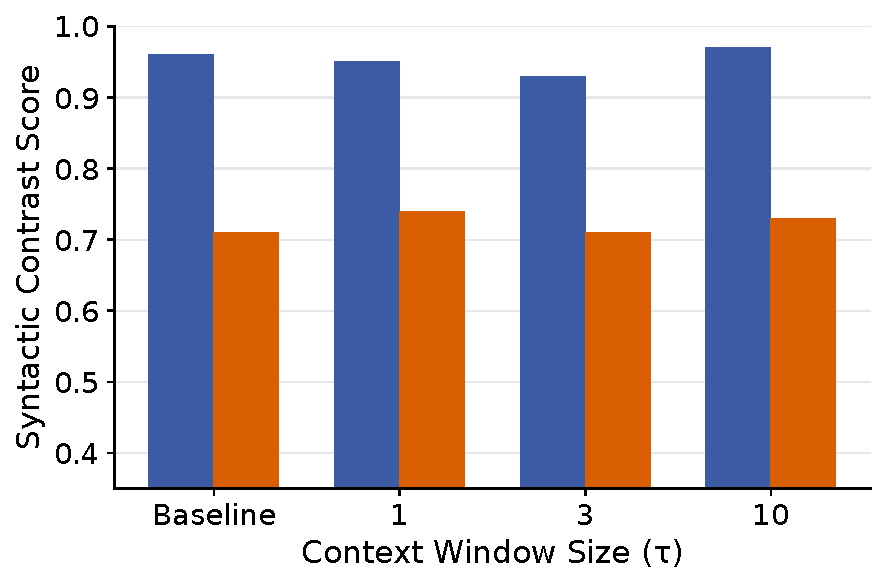
\includegraphics[width=\linewidth]{figs/paper/context_window/Neighbor1_gpt2-xl_SV_token.pdf}
    (a) SV -- token
\end{minipage}\hfill
\begin{minipage}[t]{0.32\textwidth}
    \centering
    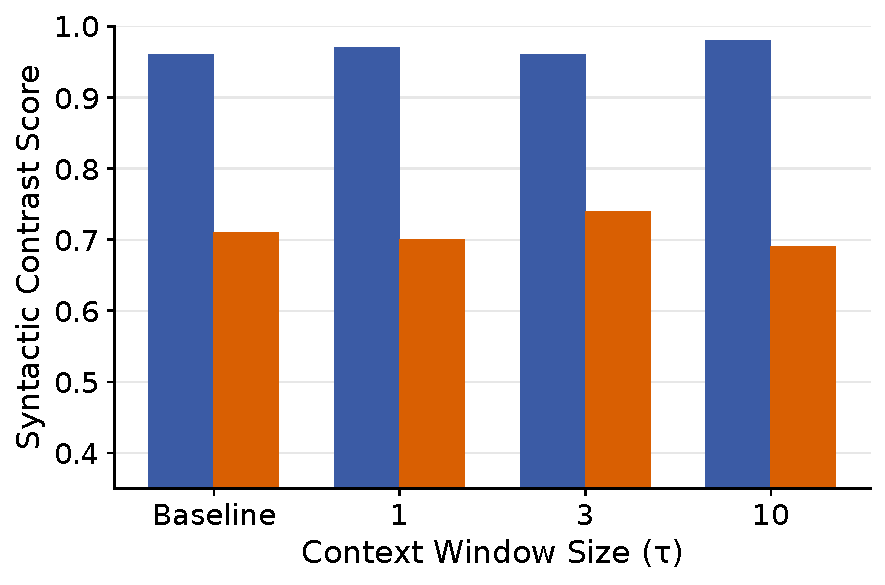
\includegraphics[width=\linewidth]{figs/paper/context_window/Neighbor1_gpt2-xl_SV_Phrase.pdf}
    (b) SV -- phrase
\end{minipage}\hfill
\begin{minipage}[t]{0.32\textwidth}
    \centering
    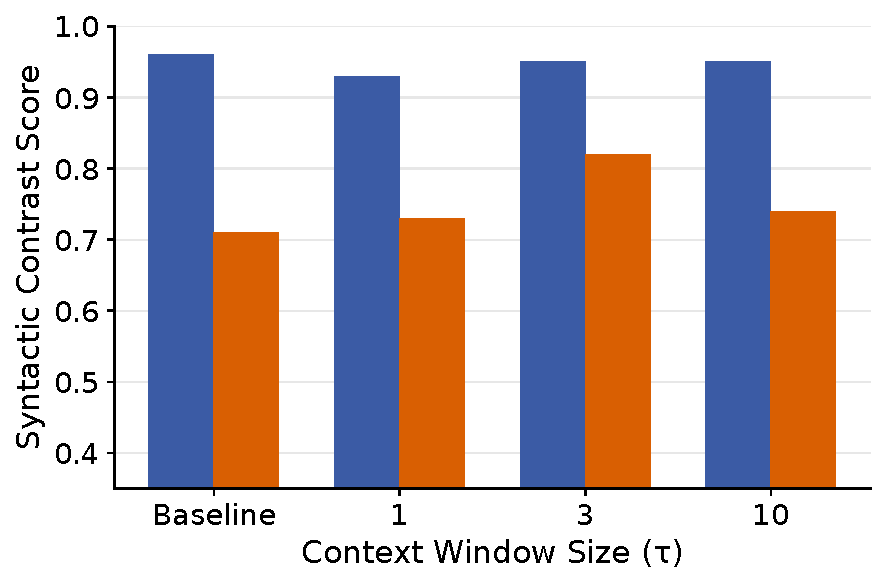
\includegraphics[width=\linewidth]{figs/paper/context_window/Neighbor1_gpt2-xl_SV_Clause.pdf}
    (c) SV -- sequence
\end{minipage}
\vspace{2mm}
\begin{minipage}[t]{0.32\textwidth}
    \centering
    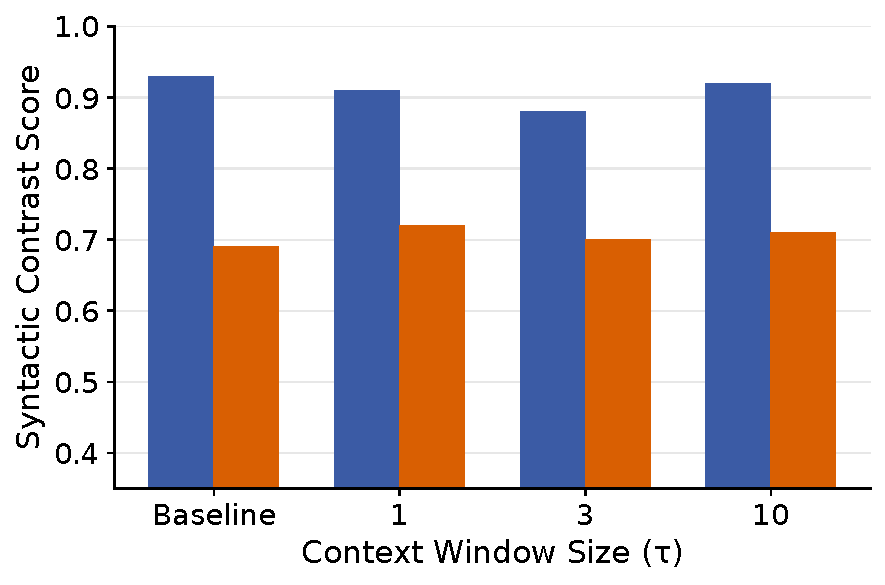
\includegraphics[width=\linewidth]{figs/paper/context_window/Neighbor1_gpt2-xl_Wh_token.pdf}
    (d) Wh -- token
\end{minipage}\hfill
\begin{minipage}[t]{0.32\textwidth}
    \centering
    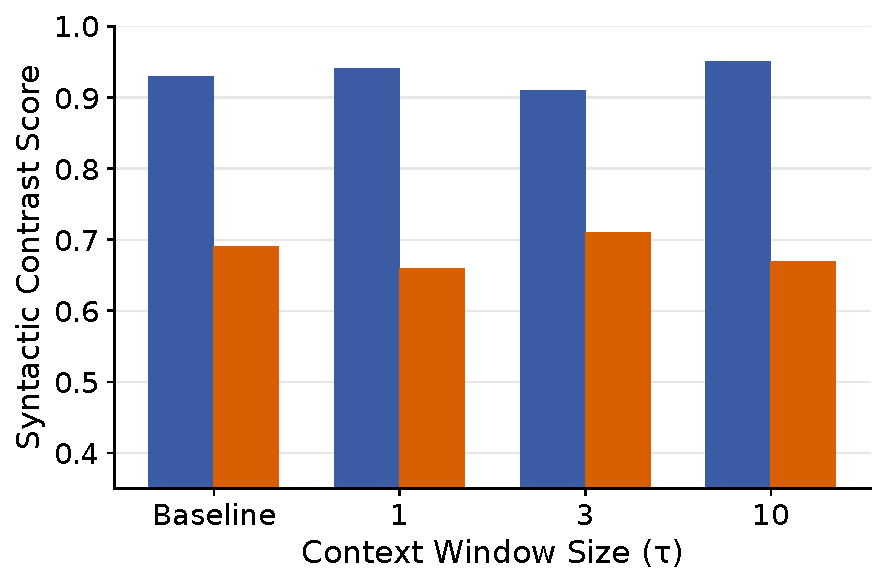
\includegraphics[width=\linewidth]{figs/paper/context_window/Neighbor1_gpt2-xl_Wh_Phrase.pdf}
    (e) Wh -- phrase
\end{minipage}\hfill
\begin{minipage}[t]{0.32\textwidth}
    \centering
    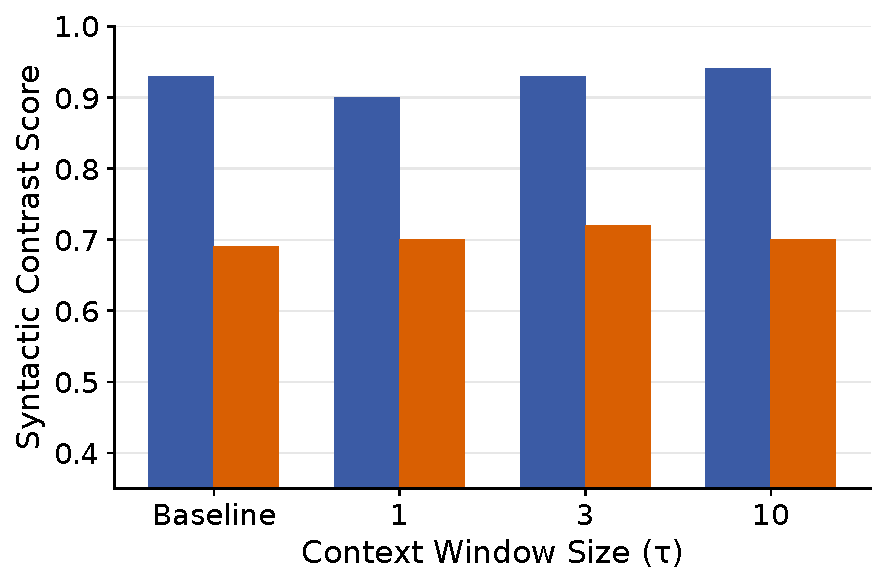
\includegraphics[width=\linewidth]{figs/paper/context_window/Neighbor1_gpt2-xl_Wh_Clause.pdf}
    (f) Wh -- sequence
\end{minipage}
\vspace{2mm}
\begin{minipage}[t]{0.32\textwidth}
    \centering
    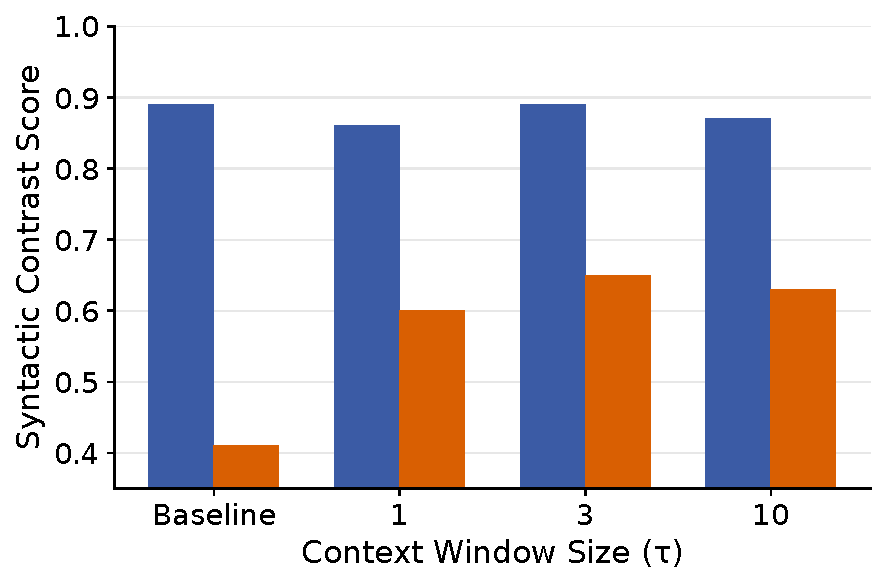
\includegraphics[width=\linewidth]{figs/paper/context_window/Neighbor1_gpt2-xl_RCs_token.pdf}
    (g) RC -- token
\end{minipage}\hfill
\begin{minipage}[t]{0.32\textwidth}
    \centering
    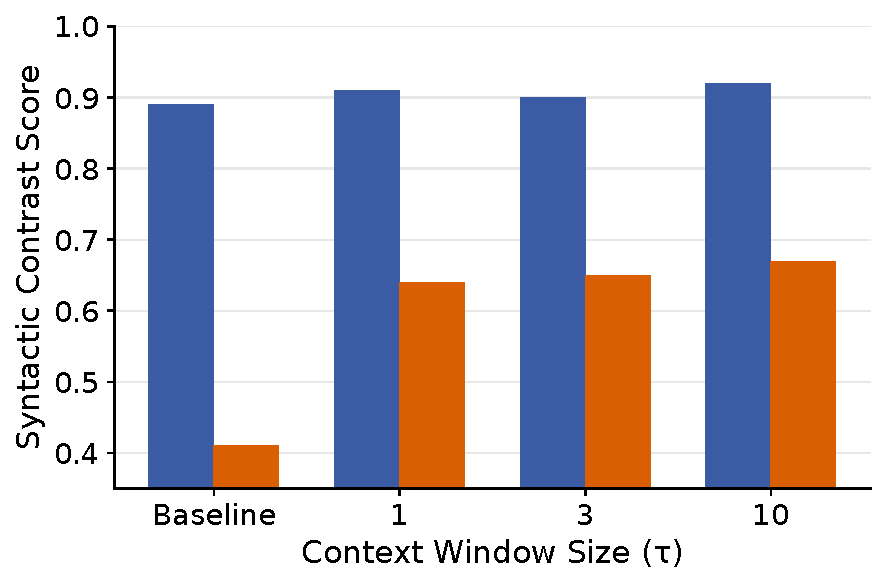
\includegraphics[width=\linewidth]{figs/paper/context_window/Neighbor1_gpt2-xl_RCs_Phrase.pdf}
    (h) RC -- phrase
\end{minipage}\hfill
\begin{minipage}[t]{0.32\textwidth}
    \centering
    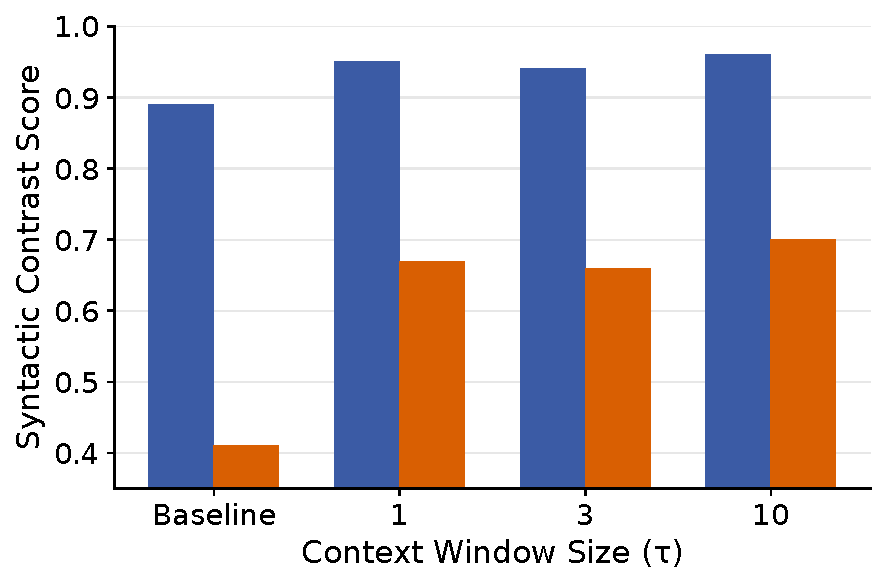
\includegraphics[width=\linewidth]{figs/paper/context_window/Neighbor1_gpt2-xl_RCs_Clause.pdf}
    (i) RC -- sequence
\end{minipage}
\caption{Effect of context window size ($\tau \in \{1,3,10\}$) for GPT-2 XL at $k=1$. Blue bars indicate high-frequency items and orange bars indicate low-frequency items; baseline results are shown for reference.}
\label{fig:app_context_gpt2xl_k1}
\end{figure*}

% ===== FIGURE: Context window, GPT-2 XL, k=1024 =====
\begin{figure*}[tp]
\centering
\begin{minipage}[t]{0.32\textwidth}
    \centering
    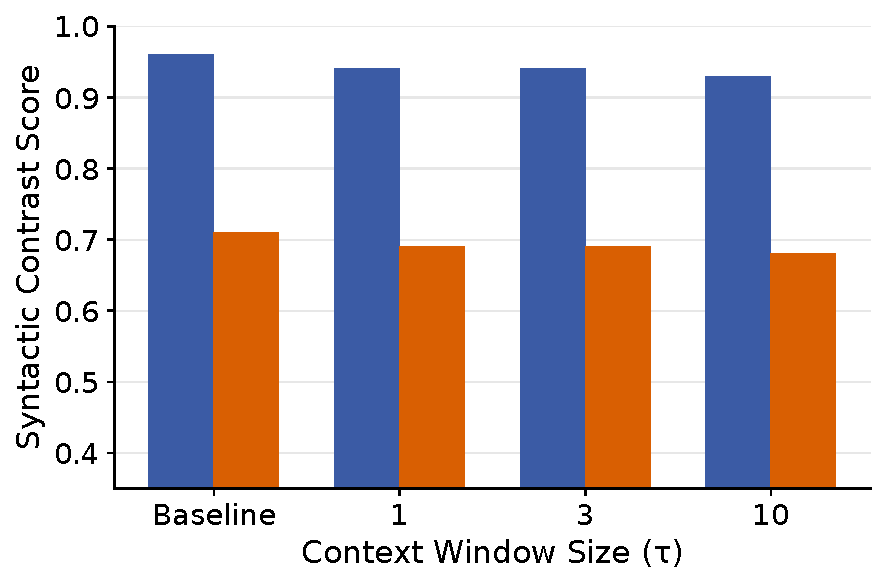
\includegraphics[width=\linewidth]{figs/paper/context_window/Neighbor1024_gpt2-xl_SV_token.pdf}
    (a) SV -- token
\end{minipage}\hfill
\begin{minipage}[t]{0.32\textwidth}
    \centering
    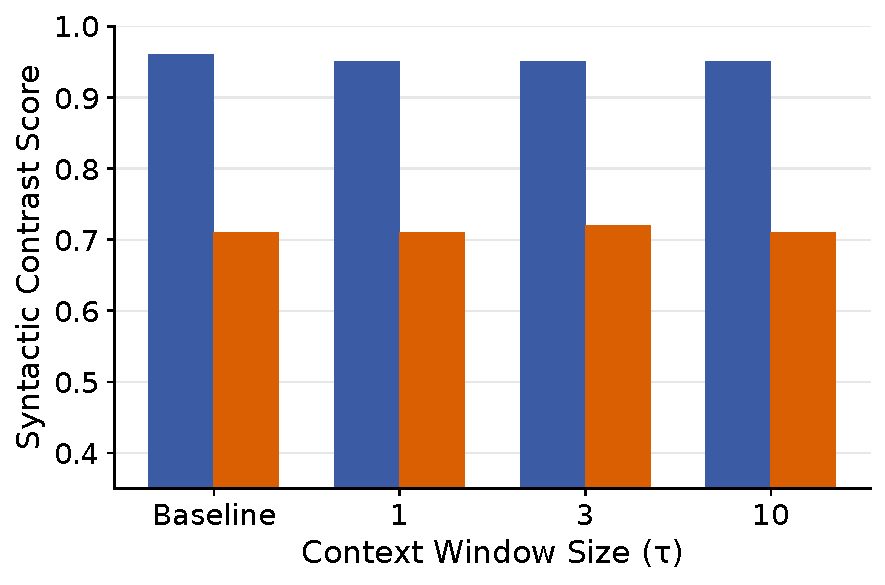
\includegraphics[width=\linewidth]{figs/paper/context_window/Neighbor1024_gpt2-xl_SV_Phrase.pdf}
    (b) SV -- phrase
\end{minipage}\hfill
\begin{minipage}[t]{0.32\textwidth}
    \centering
    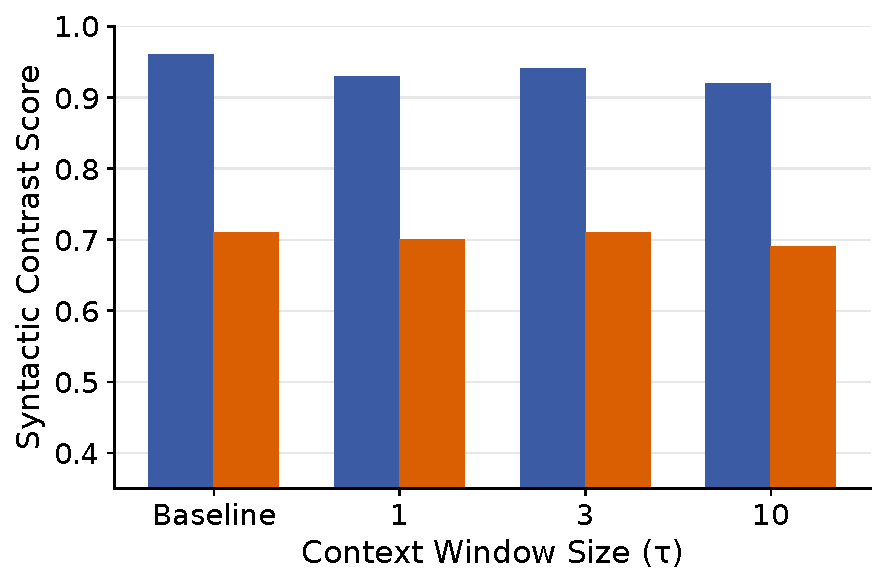
\includegraphics[width=\linewidth]{figs/paper/context_window/Neighbor1024_gpt2-xl_SV_Clause.pdf}
    (c) SV -- sequence
\end{minipage}
\vspace{2mm}
\begin{minipage}[t]{0.32\textwidth}
    \centering
    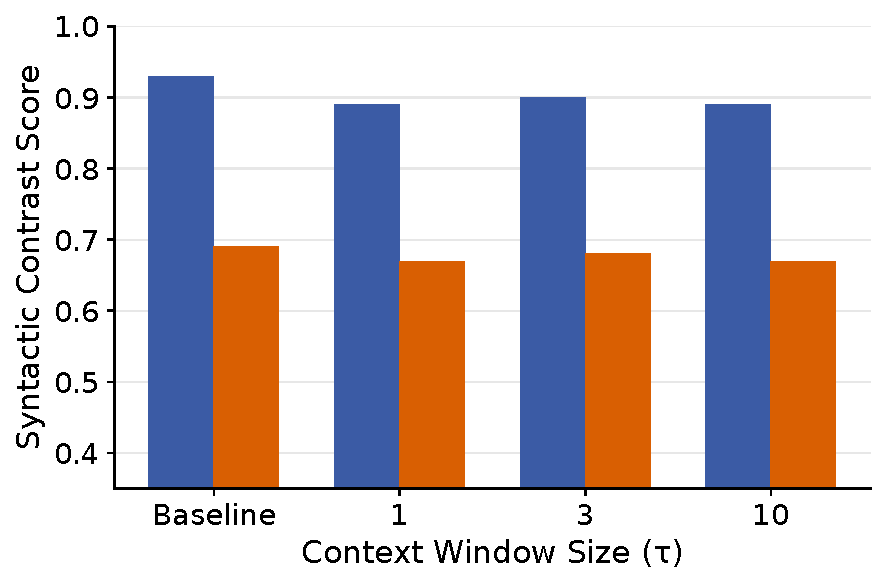
\includegraphics[width=\linewidth]{figs/paper/context_window/Neighbor1024_gpt2-xl_Wh_token.pdf}
    (d) Wh -- token
\end{minipage}\hfill
\begin{minipage}[t]{0.32\textwidth}
    \centering
    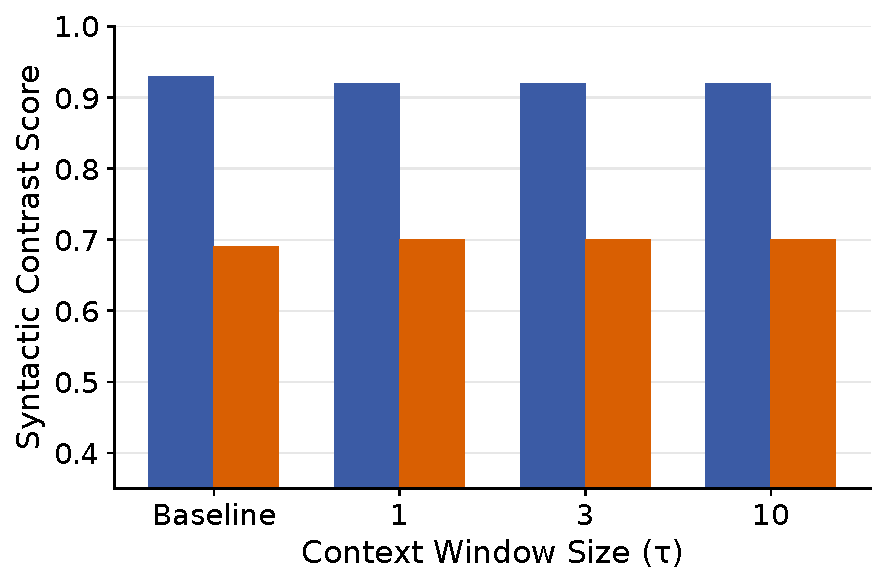
\includegraphics[width=\linewidth]{figs/paper/context_window/Neighbor1024_gpt2-xl_Wh_Phrase.pdf}
    (e) Wh -- phrase
\end{minipage}\hfill
\begin{minipage}[t]{0.32\textwidth}
    \centering
    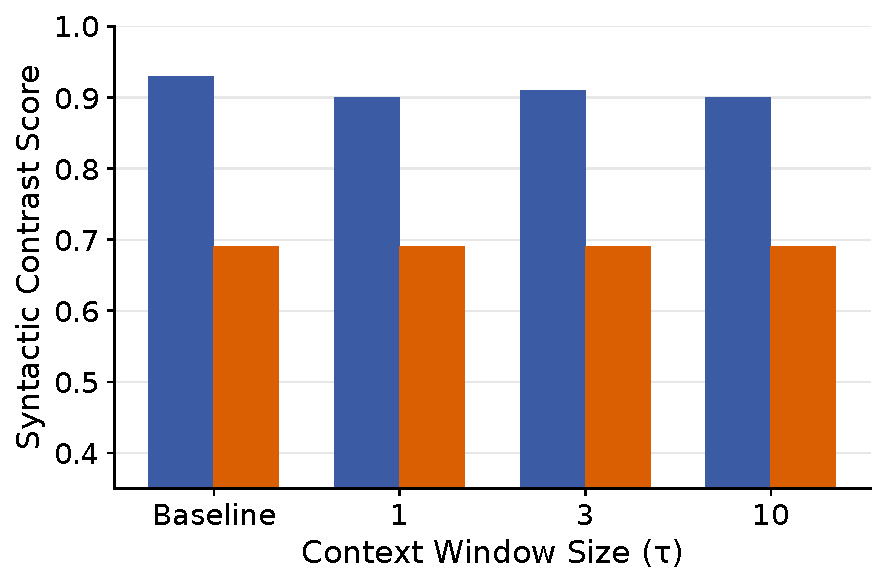
\includegraphics[width=\linewidth]{figs/paper/context_window/Neighbor1024_gpt2-xl_Wh_Clause.pdf}
    (f) Wh -- sequence
\end{minipage}
\vspace{2mm}
\begin{minipage}[t]{0.32\textwidth}
    \centering
    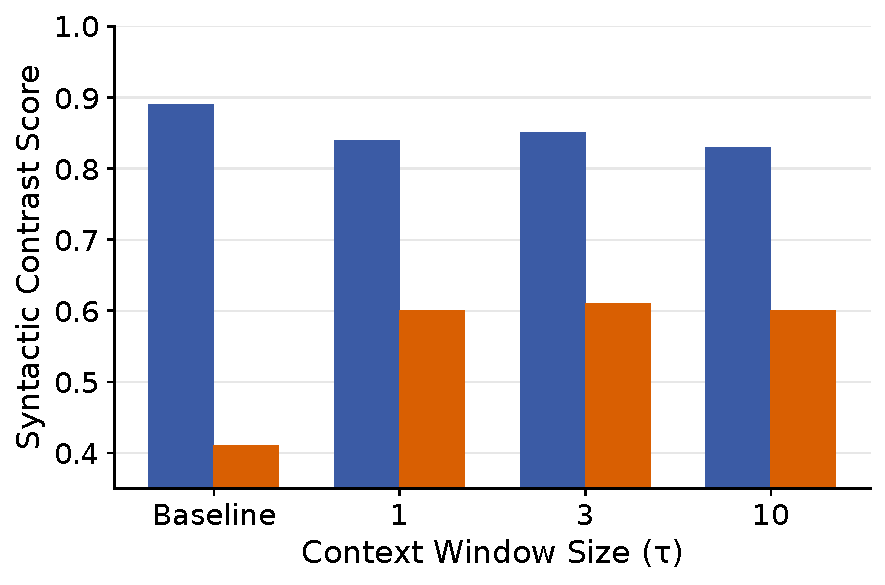
\includegraphics[width=\linewidth]{figs/paper/context_window/Neighbor1024_gpt2-xl_RCs_token.pdf}
    (g) RC -- token
\end{minipage}\hfill
\begin{minipage}[t]{0.32\textwidth}
    \centering
    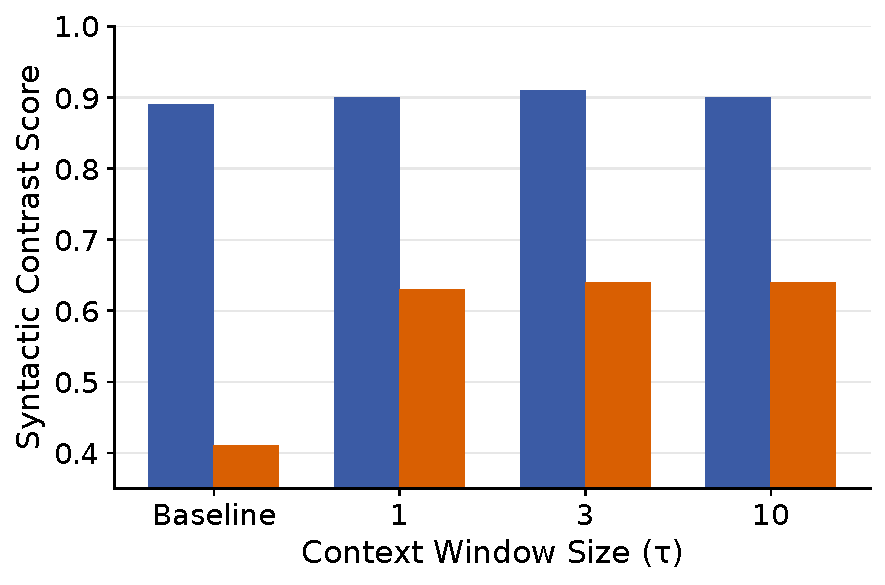
\includegraphics[width=\linewidth]{figs/paper/context_window/Neighbor1024_gpt2-xl_RCs_Phrase.pdf}
    (h) RC -- phrase
\end{minipage}\hfill
\begin{minipage}[t]{0.32\textwidth}
    \centering
    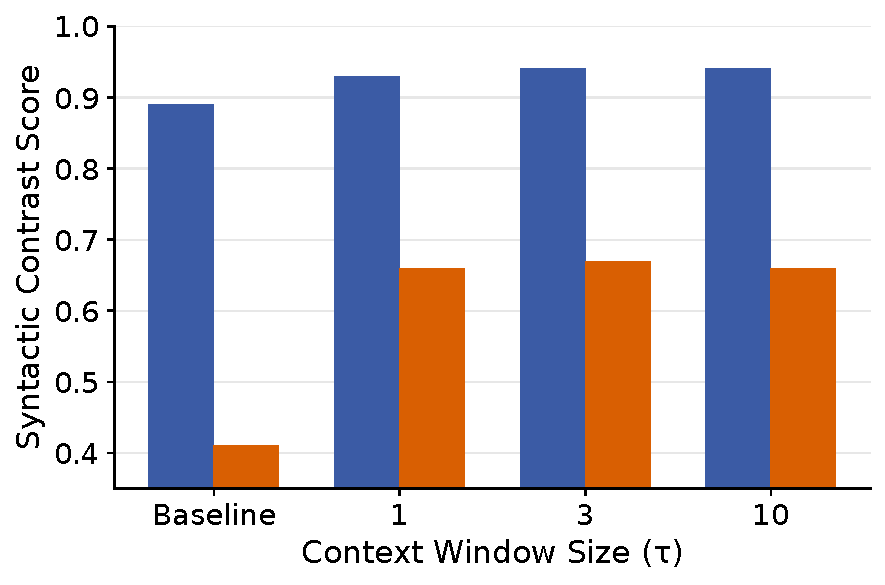
\includegraphics[width=\linewidth]{figs/paper/context_window/Neighbor1024_gpt2-xl_RCs_Clause.pdf}
    (i) RC -- sequence
\end{minipage}
\caption{Effect of context window size ($\tau \in \{1,3,10\}$) for GPT-2 XL at $k=1024$. Blue bars indicate high-frequency items and orange bars indicate low-frequency items; baseline results are shown for reference.}
\label{fig:app_context_gpt2xl_k1024}
\end{figure*}

% ===== FIGURE: Context window, Bounded-data, k=1 =====
\begin{figure*}[tp]
\centering
\begin{minipage}[t]{0.32\textwidth}
    \centering
    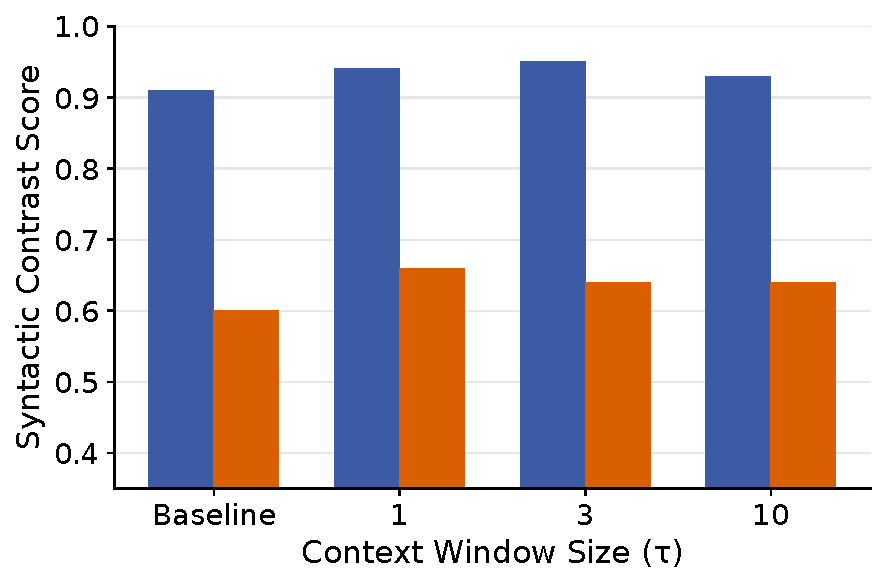
\includegraphics[width=\linewidth]{figs/paper/context_window/Neighbor1_child-realistic_SV_token.pdf}
    (a) SV -- token
\end{minipage}\hfill
\begin{minipage}[t]{0.32\textwidth}
    \centering
    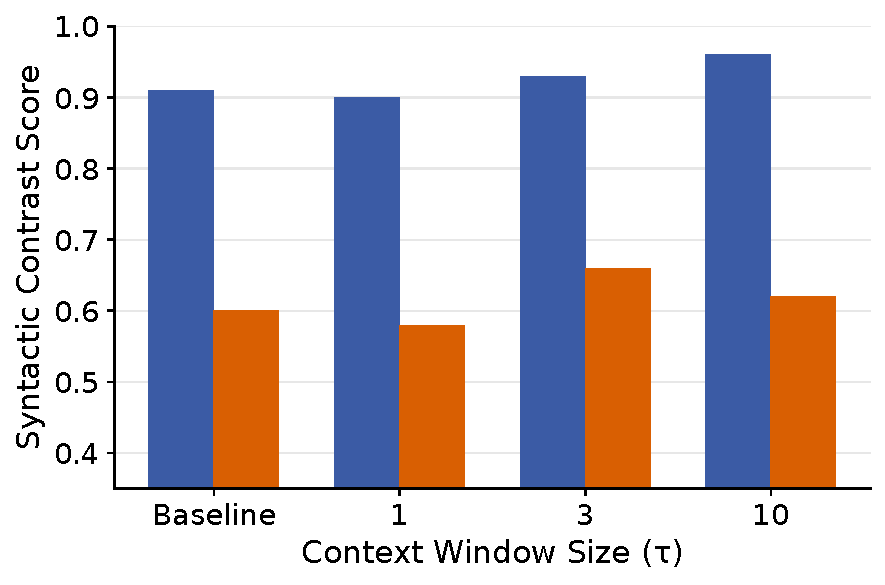
\includegraphics[width=\linewidth]{figs/paper/context_window/Neighbor1_child-realistic_SV_Phrase.pdf}
    (b) SV -- phrase
\end{minipage}\hfill
\begin{minipage}[t]{0.32\textwidth}
    \centering
    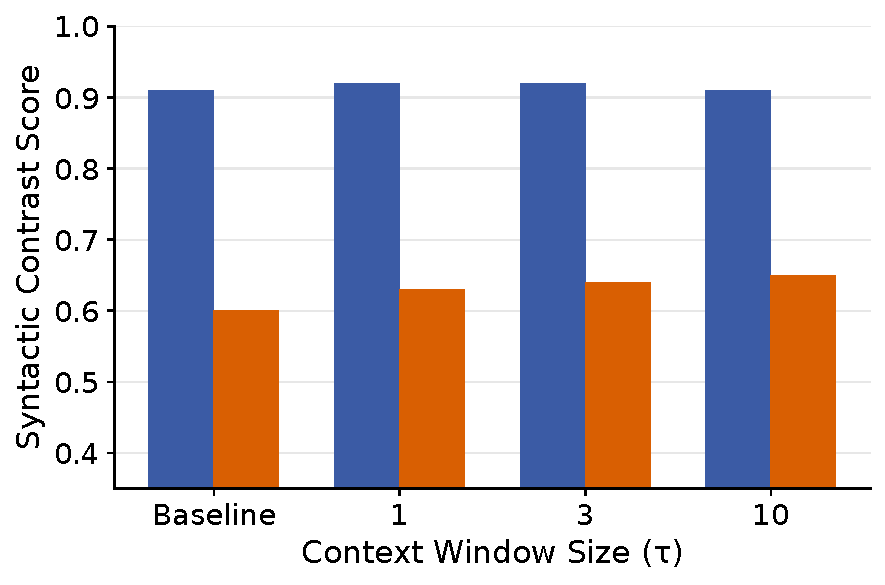
\includegraphics[width=\linewidth]{figs/paper/context_window/Neighbor1_child-realistic_SV_Clause.pdf}
    (c) SV -- sequence
\end{minipage}
\vspace{2mm}
\begin{minipage}[t]{0.32\textwidth}
    \centering
    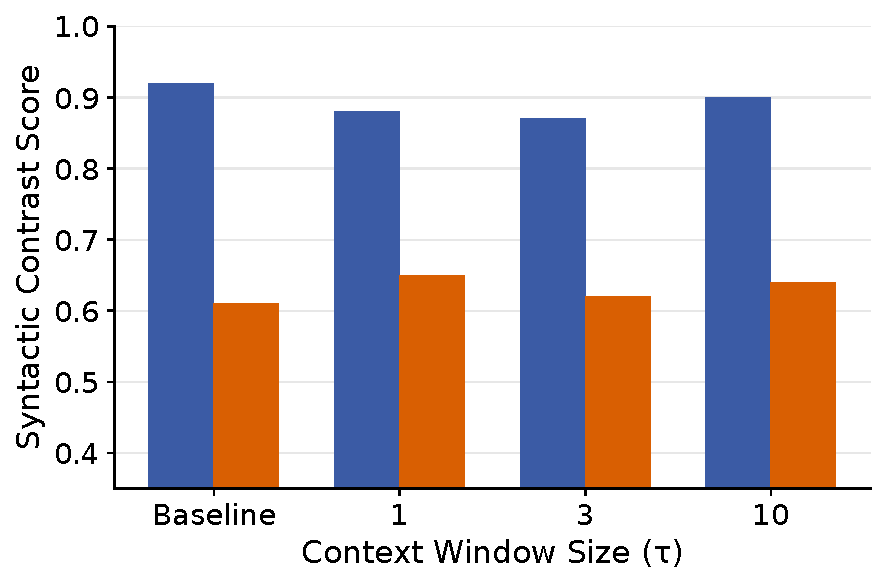
\includegraphics[width=\linewidth]{figs/paper/context_window/Neighbor1_child-realistic_Wh_token.pdf}
    (d) Wh -- token
\end{minipage}\hfill
\begin{minipage}[t]{0.32\textwidth}
    \centering
    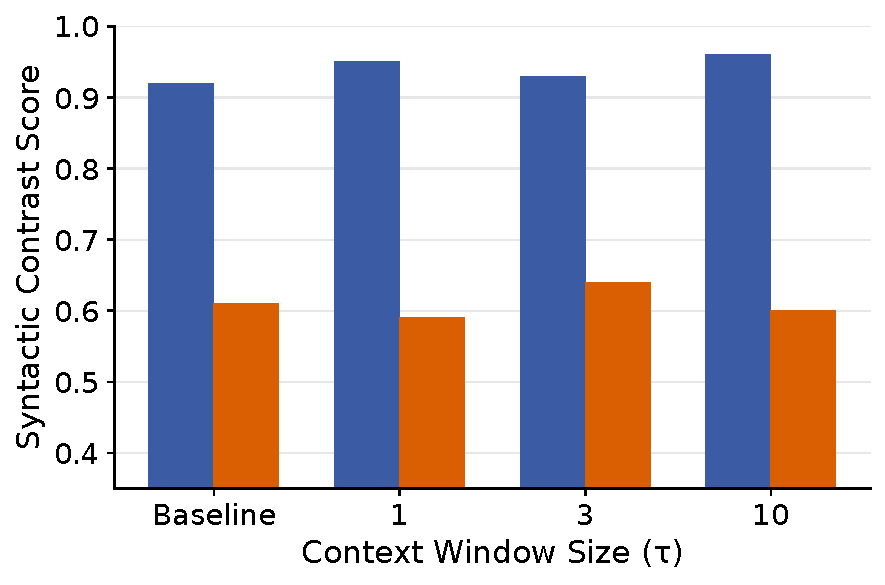
\includegraphics[width=\linewidth]{figs/paper/context_window/Neighbor1_child-realistic_Wh_Phrase.pdf}
    (e) Wh -- phrase
\end{minipage}\hfill
\begin{minipage}[t]{0.32\textwidth}
    \centering
    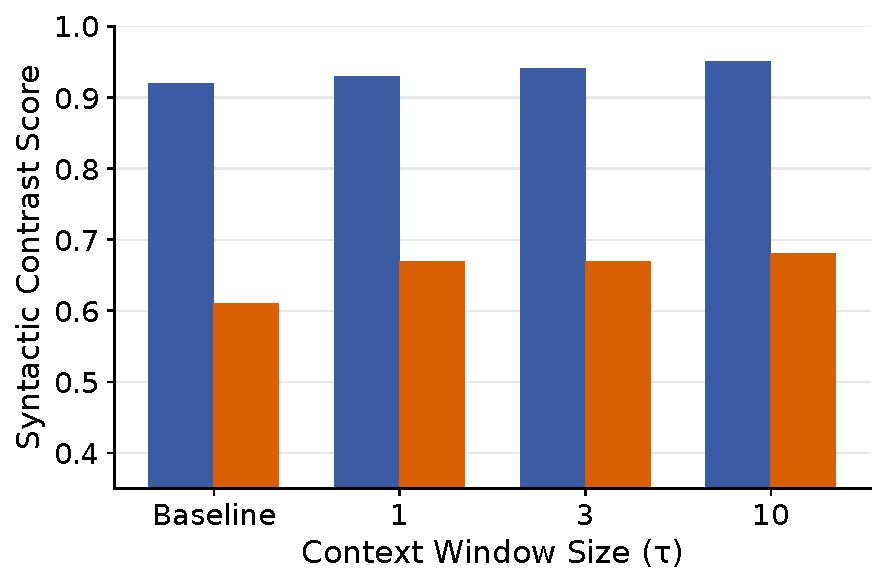
\includegraphics[width=\linewidth]{figs/paper/context_window/Neighbor1_child-realistic_Wh_Clause.pdf}
    (f) Wh -- sequence
\end{minipage}
\vspace{2mm}
\begin{minipage}[t]{0.32\textwidth}
    \centering
    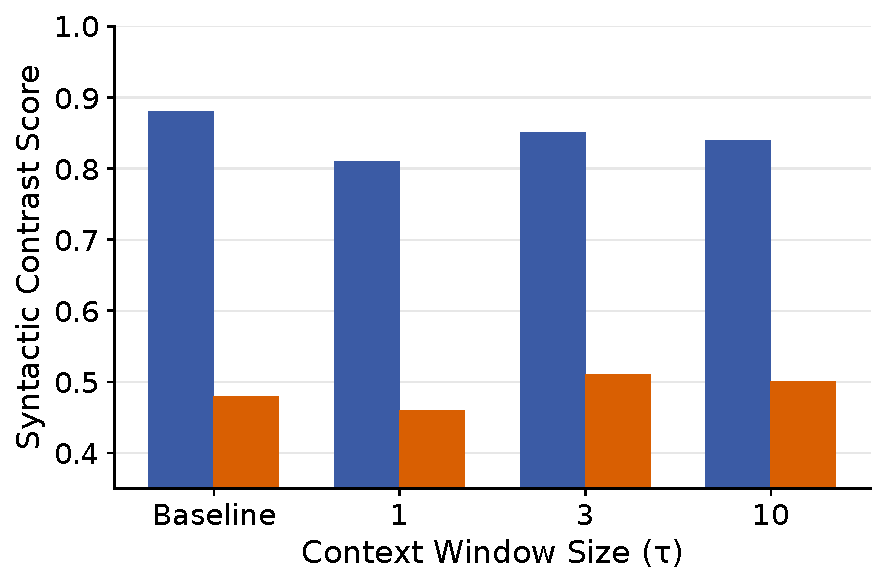
\includegraphics[width=\linewidth]{figs/paper/context_window/Neighbor1_child-realistic_RCs_token.pdf}
    (g) RC -- token
\end{minipage}\hfill
\begin{minipage}[t]{0.32\textwidth}
    \centering
    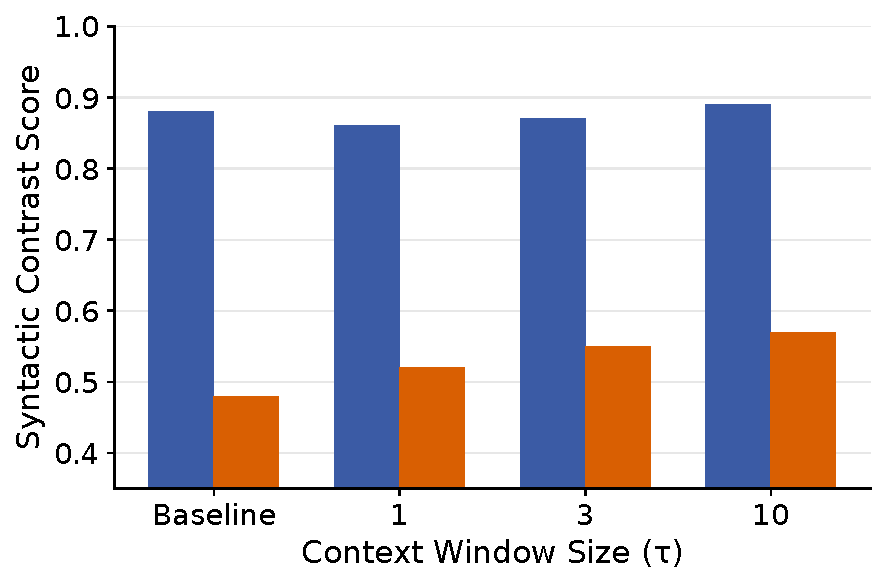
\includegraphics[width=\linewidth]{figs/paper/context_window/Neighbor1_child-realistic_RCs_Phrase.pdf}
    (h) RC -- phrase
\end{minipage}\hfill
\begin{minipage}[t]{0.32\textwidth}
    \centering
    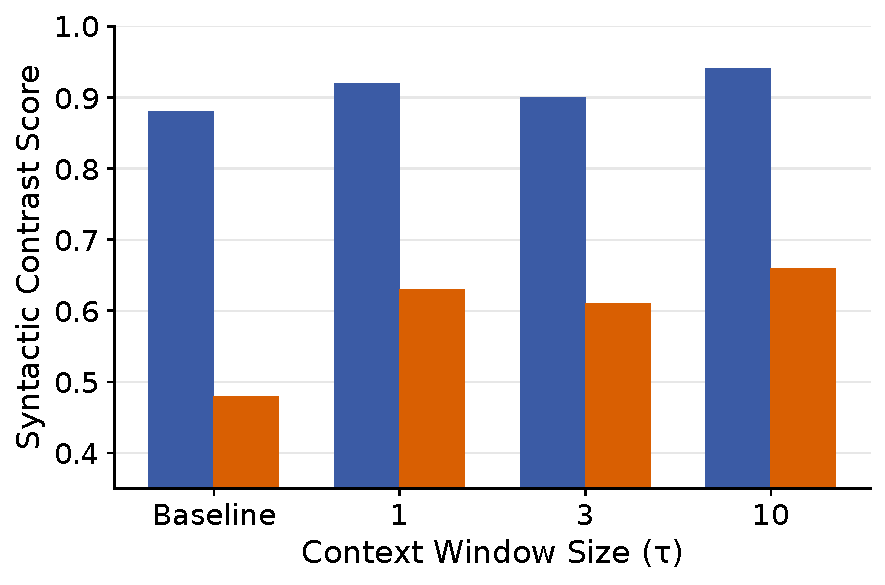
\includegraphics[width=\linewidth]{figs/paper/context_window/Neighbor1_child-realistic_RCs_Clause.pdf}
    (i) RC -- sequence
\end{minipage}
\caption{Effect of context window size ($\tau \in \{1,3,10\}$) for the bounded-data model at $k=1$. Blue bars indicate high-frequency items and orange bars indicate low-frequency items; baseline results are shown for reference.}
\label{fig:app_context_child_k1}
\end{figure*}

% ===== FIGURE: Context window, Bounded-data, k=1024 =====
\begin{figure*}[tp]
\centering
\begin{minipage}[t]{0.32\textwidth}
    \centering
    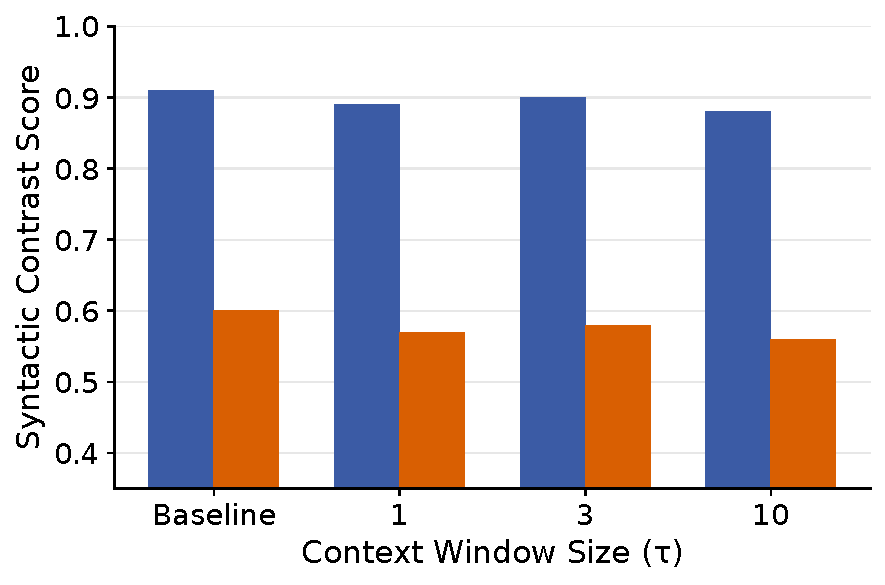
\includegraphics[width=\linewidth]{figs/paper/context_window/Neighbor1024_child-realistic_SV_token.pdf}
    (a) SV -- token
\end{minipage}\hfill
\begin{minipage}[t]{0.32\textwidth}
    \centering
    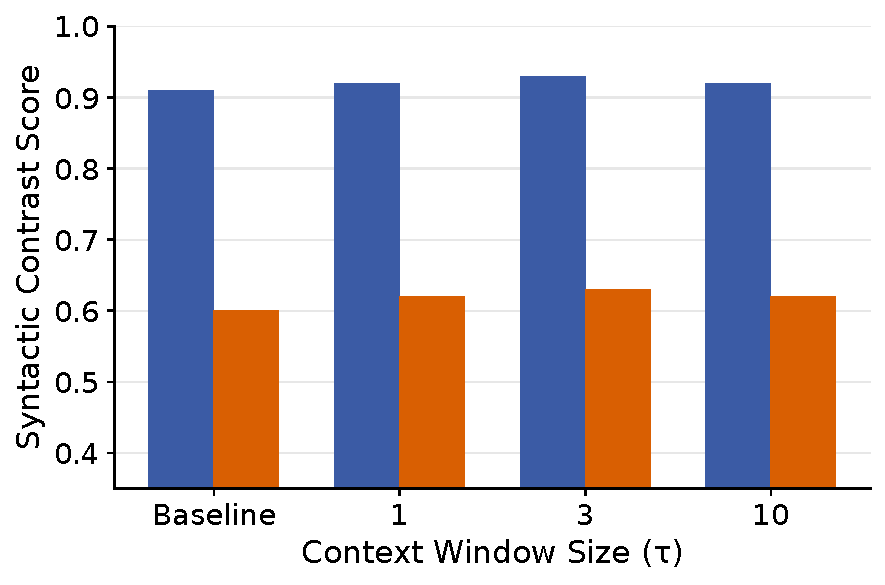
\includegraphics[width=\linewidth]{figs/paper/context_window/Neighbor1024_child-realistic_SV_Phrase.pdf}
    (b) SV -- phrase
\end{minipage}\hfill
\begin{minipage}[t]{0.32\textwidth}
    \centering
    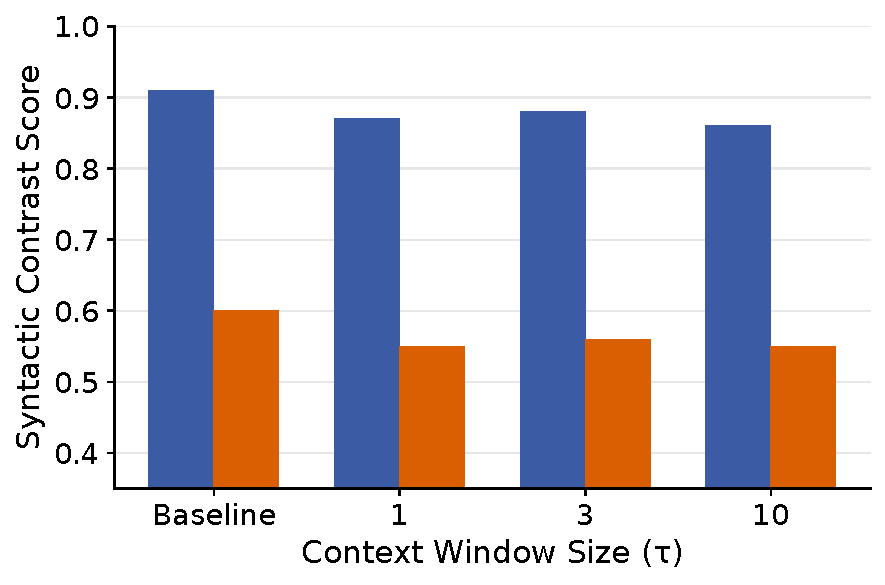
\includegraphics[width=\linewidth]{figs/paper/context_window/Neighbor1024_child-realistic_SV_Clause.pdf}
    (c) SV -- sequence
\end{minipage}
\vspace{2mm}
\begin{minipage}[t]{0.32\textwidth}
    \centering
    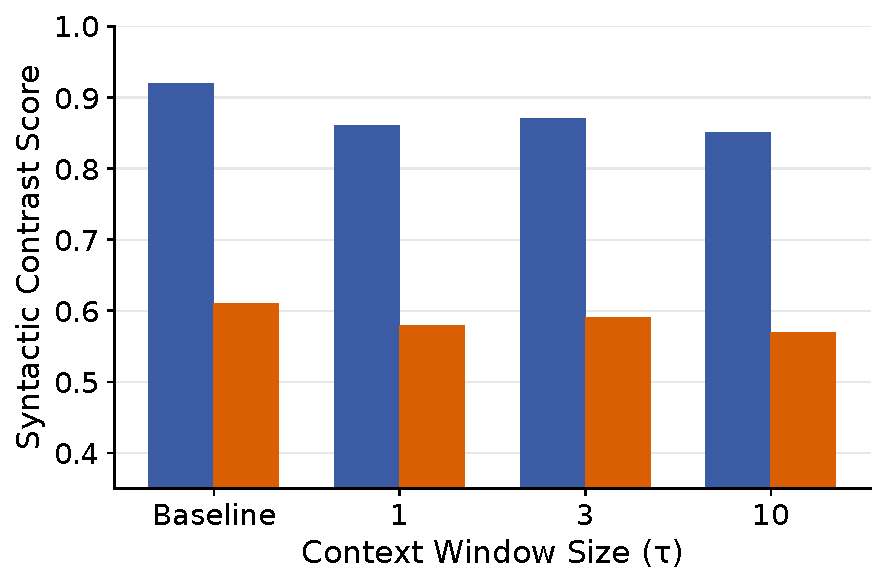
\includegraphics[width=\linewidth]{figs/paper/context_window/Neighbor1024_child-realistic_Wh_token.pdf}
    (d) Wh -- token
\end{minipage}\hfill
\begin{minipage}[t]{0.32\textwidth}
    \centering
    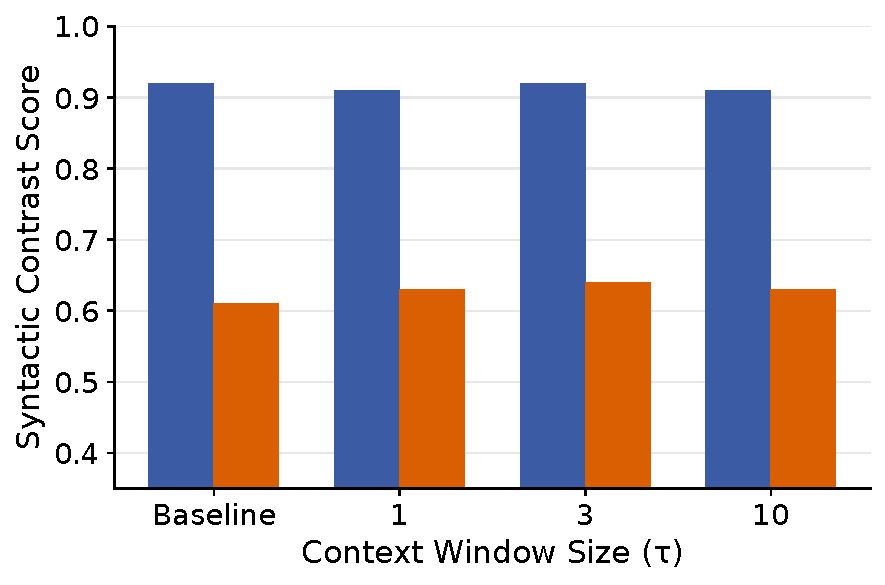
\includegraphics[width=\linewidth]{figs/paper/context_window/Neighbor1024_child-realistic_Wh_Phrase.pdf}
    (e) Wh -- phrase
\end{minipage}\hfill
\begin{minipage}[t]{0.32\textwidth}
    \centering
    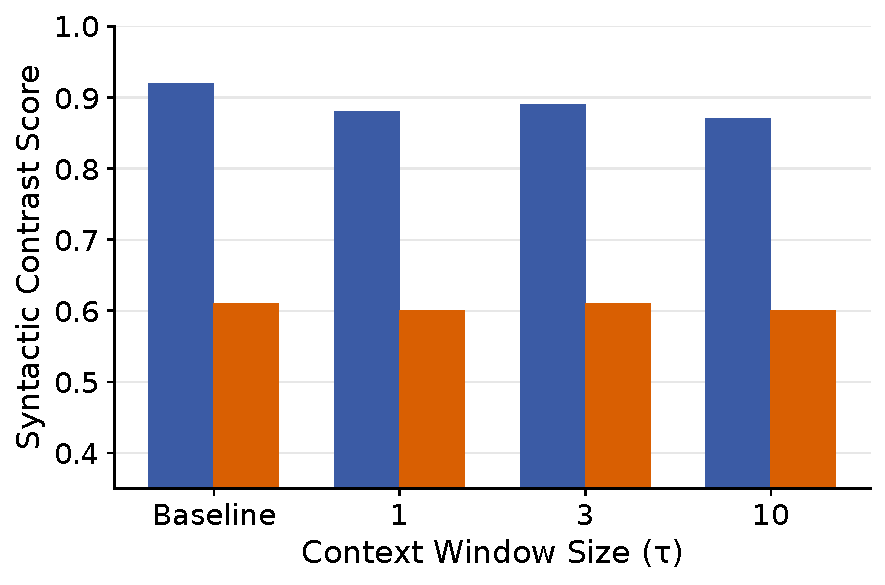
\includegraphics[width=\linewidth]{figs/paper/context_window/Neighbor1024_child-realistic_Wh_Clause.pdf}
    (f) Wh -- sequence
\end{minipage}
\vspace{2mm}
\begin{minipage}[t]{0.32\textwidth}
    \centering
    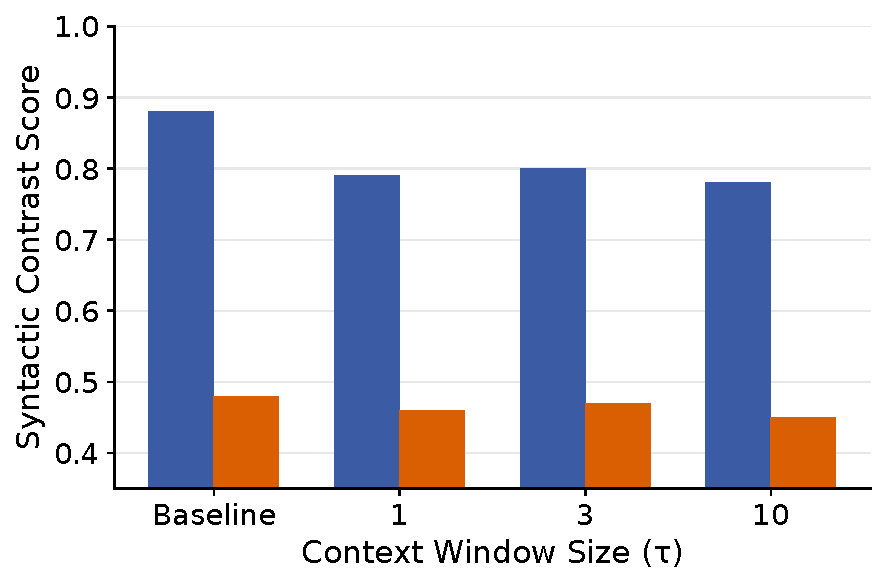
\includegraphics[width=\linewidth]{figs/paper/context_window/Neighbor1024_child-realistic_RCs_token.pdf}
    (g) RC -- token
\end{minipage}\hfill
\begin{minipage}[t]{0.32\textwidth}
    \centering
    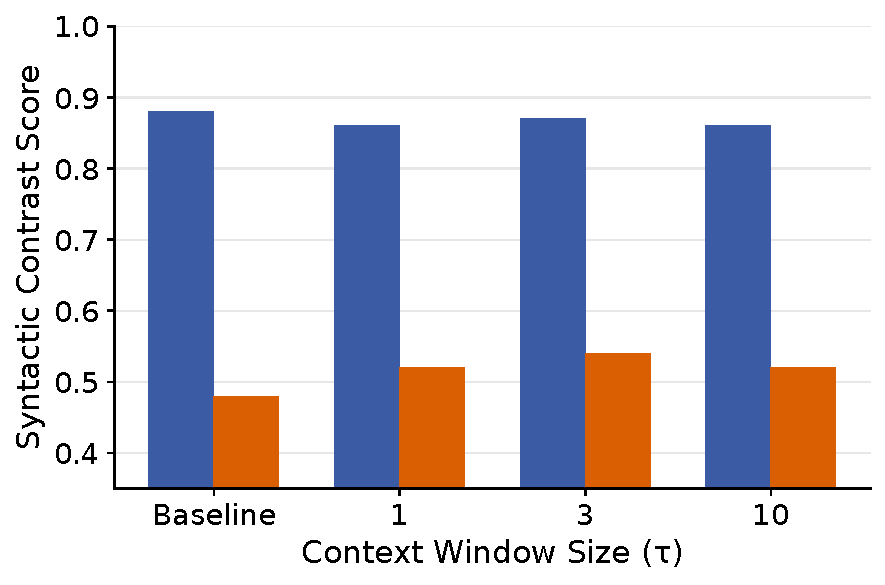
\includegraphics[width=\linewidth]{figs/paper/context_window/Neighbor1024_child-realistic_RCs_Phrase.pdf}
    (h) RC -- phrase
\end{minipage}\hfill
\begin{minipage}[t]{0.32\textwidth}
    \centering
    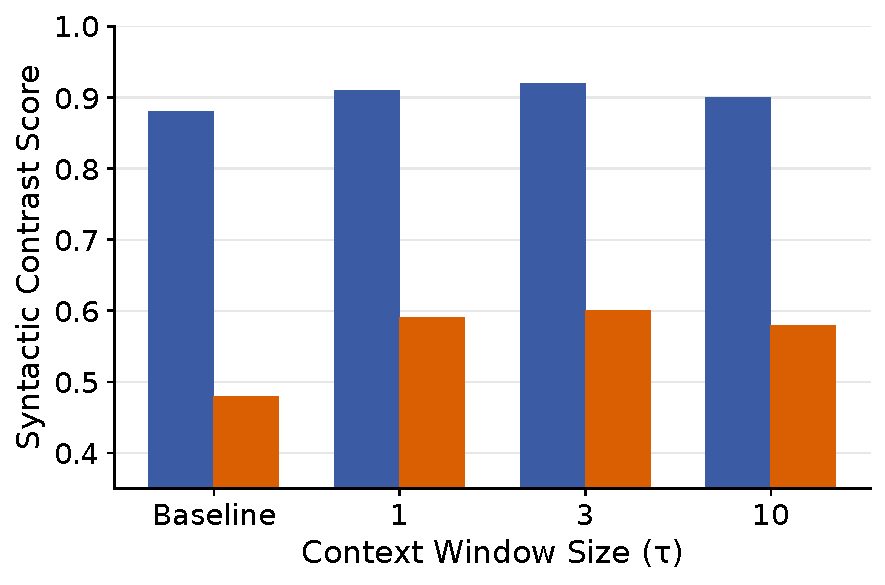
\includegraphics[width=\linewidth]{figs/paper/context_window/Neighbor1024_child-realistic_RCs_Clause.pdf}
    (i) RC -- sequence
\end{minipage}
\caption{Effect of context window size ($\tau \in \{1,3,10\}$) for the bounded-data model at $k=1024$. Blue bars indicate high-frequency items and orange bars indicate low-frequency items; baseline results are shown for reference.}
\label{fig:app_context_child_k1024}
\end{figure*}

% ===== FIGURE: Neighbor count, GPT-2 XL, tau=1 =====
\begin{figure*}[tp]
\centering
\begin{minipage}[t]{0.32\textwidth}
    \centering
    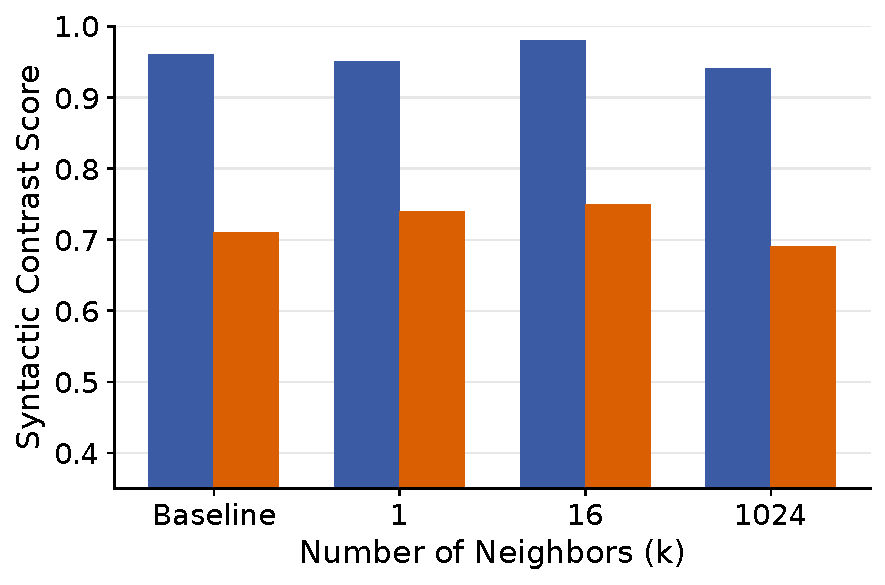
\includegraphics[width=\linewidth]{figs/paper/neighbor/Context1_gpt2-xl_SV_token.pdf}
    (a) SV -- token
\end{minipage}\hfill
\begin{minipage}[t]{0.32\textwidth}
    \centering
    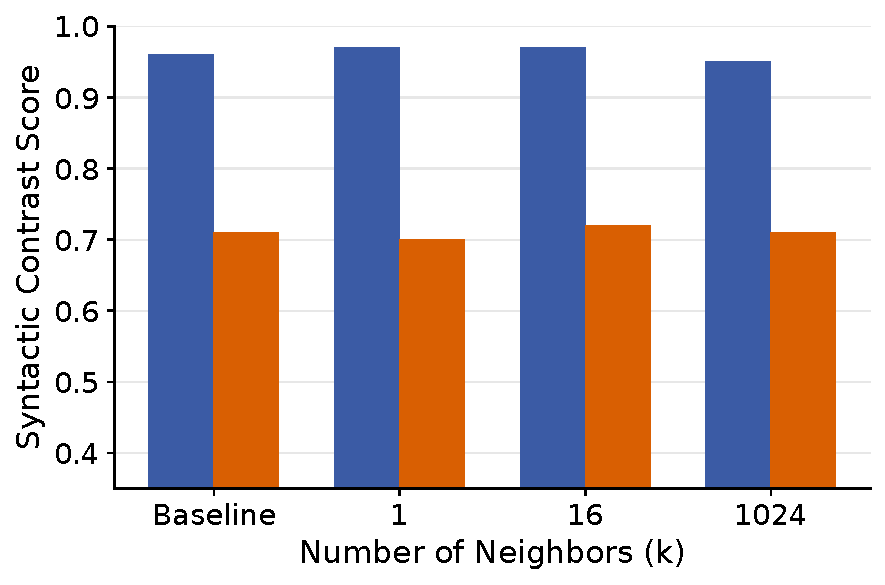
\includegraphics[width=\linewidth]{figs/paper/neighbor/Context1_gpt2-xl_SV_Phrase.pdf}
    (b) SV -- phrase
\end{minipage}\hfill
\begin{minipage}[t]{0.32\textwidth}
    \centering
    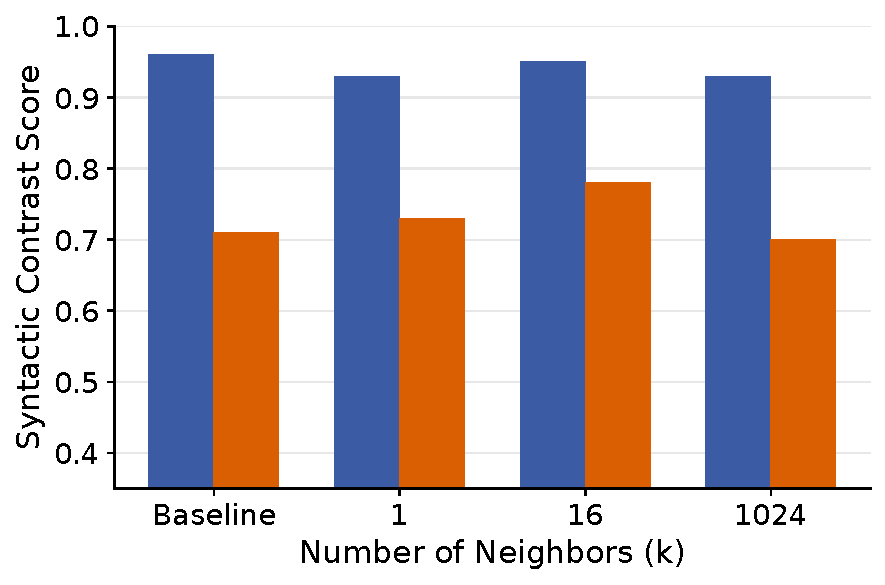
\includegraphics[width=\linewidth]{figs/paper/neighbor/Context1_gpt2-xl_SV_Clause.pdf}
    (c) SV -- sequence
\end{minipage}
\vspace{2mm}
\begin{minipage}[t]{0.32\textwidth}
    \centering
    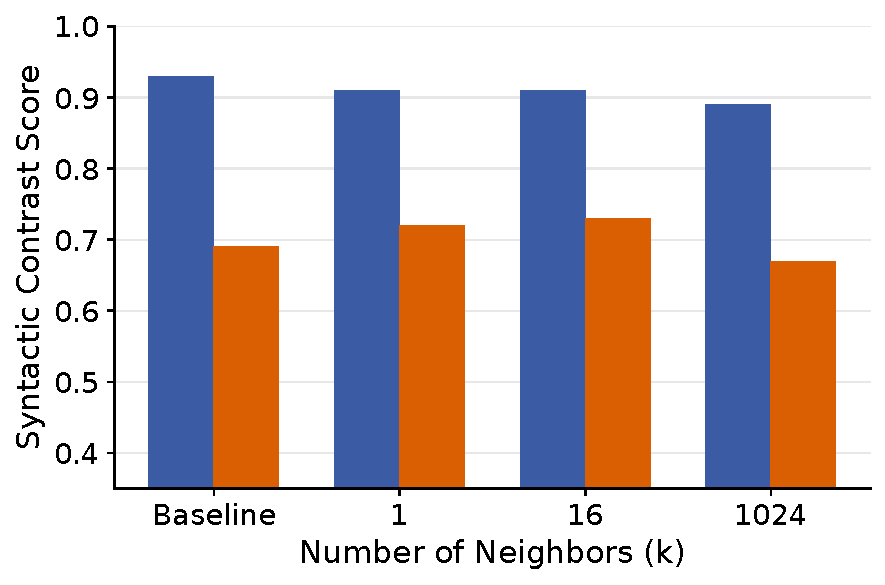
\includegraphics[width=\linewidth]{figs/paper/neighbor/Context1_gpt2-xl_Wh_token.pdf}
    (d) Wh -- token
\end{minipage}\hfill
\begin{minipage}[t]{0.32\textwidth}
    \centering
    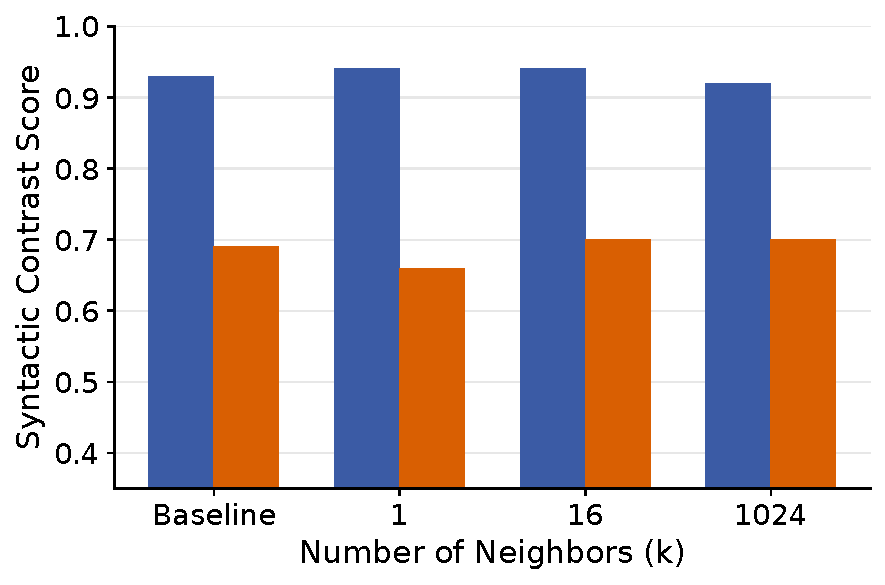
\includegraphics[width=\linewidth]{figs/paper/neighbor/Context1_gpt2-xl_Wh_Phrase.pdf}
    (e) Wh -- phrase
\end{minipage}\hfill
\begin{minipage}[t]{0.32\textwidth}
    \centering
    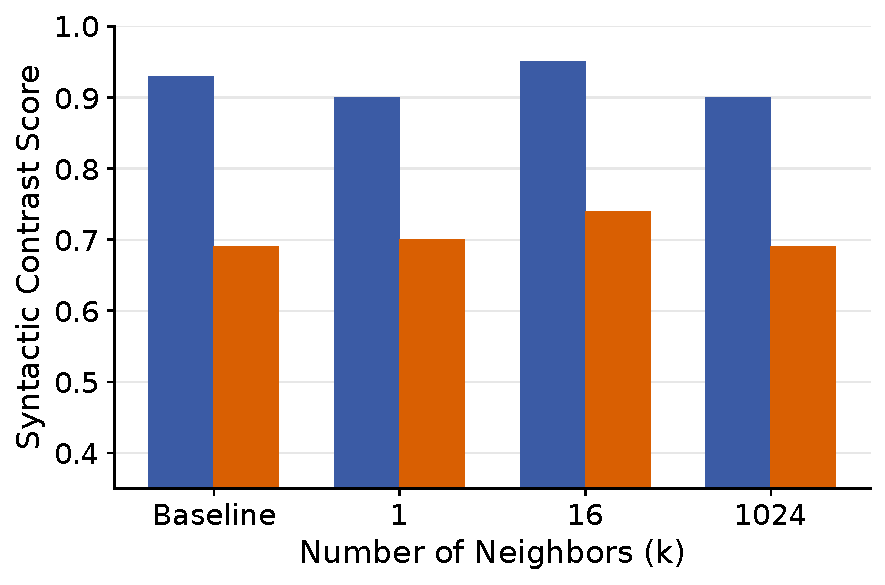
\includegraphics[width=\linewidth]{figs/paper/neighbor/Context1_gpt2-xl_Wh_Clause.pdf}
    (f) Wh -- sequence
\end{minipage}
\vspace{2mm}
\begin{minipage}[t]{0.32\textwidth}
    \centering
    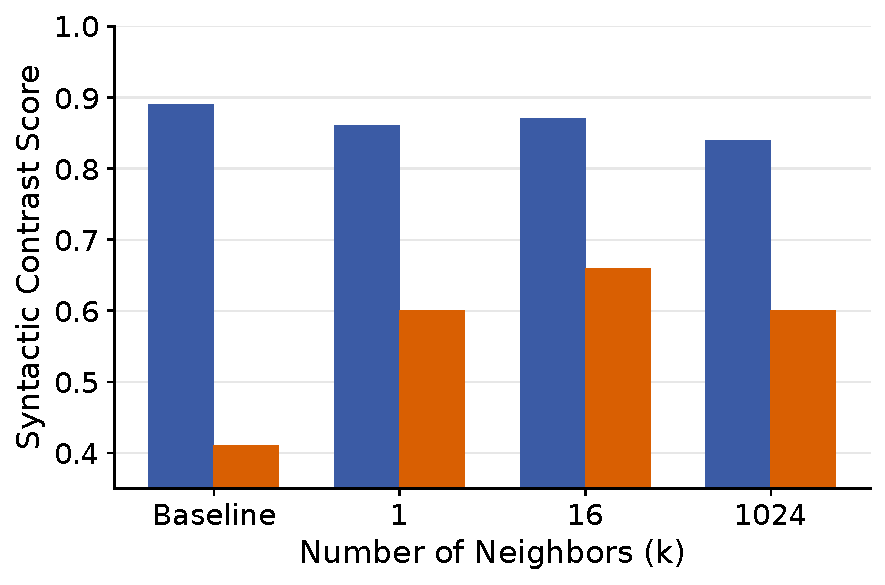
\includegraphics[width=\linewidth]{figs/paper/neighbor/Context1_gpt2-xl_RCs_token.pdf}
    (g) RC -- token
\end{minipage}\hfill
\begin{minipage}[t]{0.32\textwidth}
    \centering
    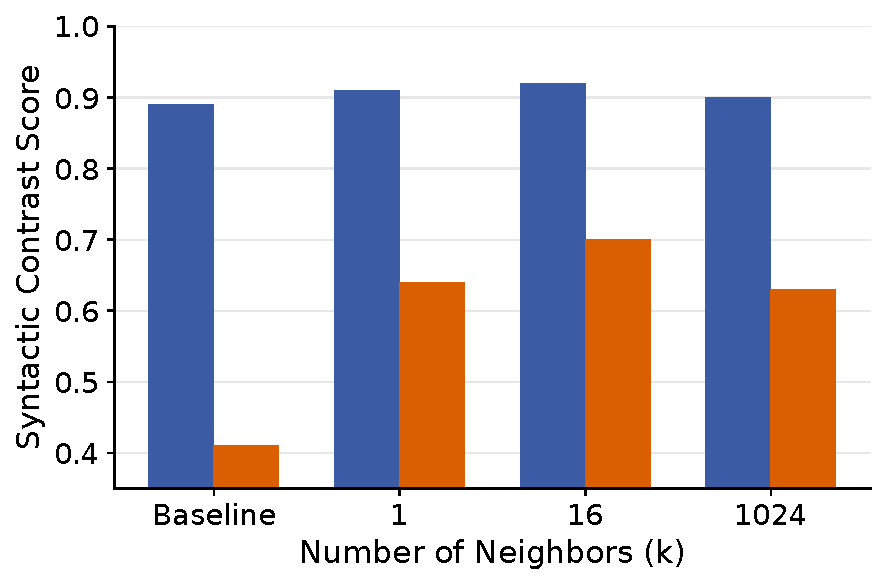
\includegraphics[width=\linewidth]{figs/paper/neighbor/Context1_gpt2-xl_RCs_Phrase.pdf}
    (h) RC -- phrase
\end{minipage}\hfill
\begin{minipage}[t]{0.32\textwidth}
    \centering
    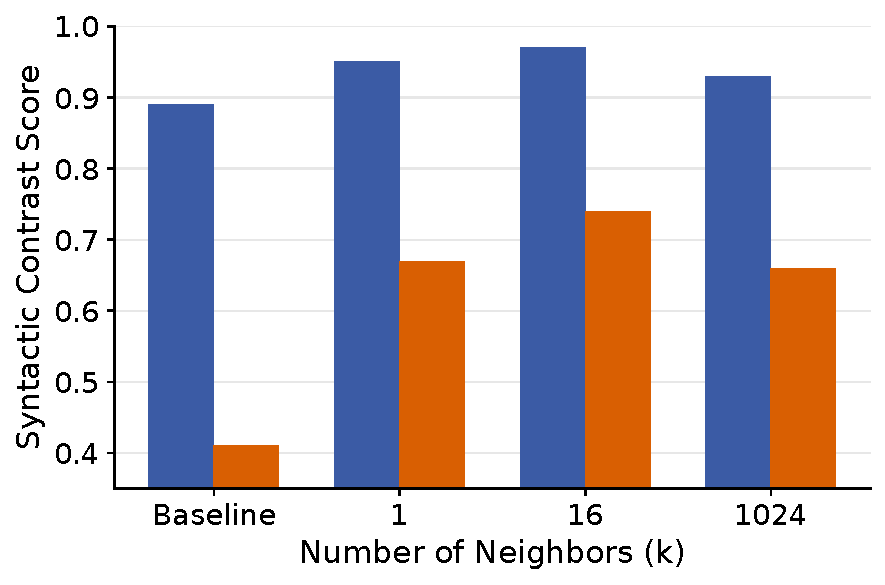
\includegraphics[width=\linewidth]{figs/paper/neighbor/Context1_gpt2-xl_RCs_Clause.pdf}
    (i) RC -- sequence
\end{minipage}
\caption{Effect of number of retrieved neighbors ($k \in \{1,16,1024\}$) for GPT-2 XL at $\tau=1$. Blue bars indicate high-frequency items and orange bars indicate low-frequency items; baseline results are shown for reference.}
\label{fig:app_neighbor_gpt2xl_tau1}
\end{figure*}

% ===== FIGURE: Neighbor count, GPT-2 XL, tau=10 =====
\begin{figure*}[tp]
\centering
\begin{minipage}[t]{0.32\textwidth}
    \centering
    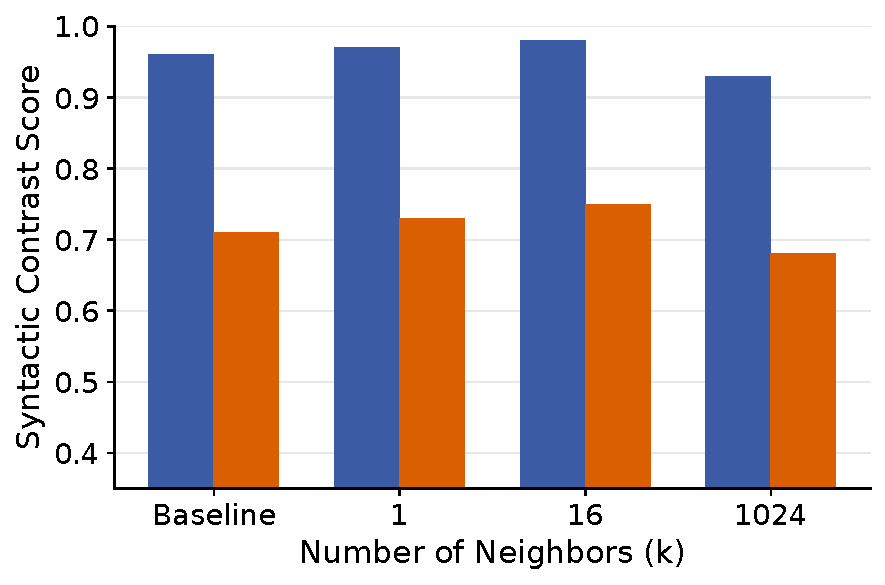
\includegraphics[width=\linewidth]{figs/paper/neighbor/Context10_gpt2-xl_SV_token.pdf}
    (a) SV -- token
\end{minipage}\hfill
\begin{minipage}[t]{0.32\textwidth}
    \centering
    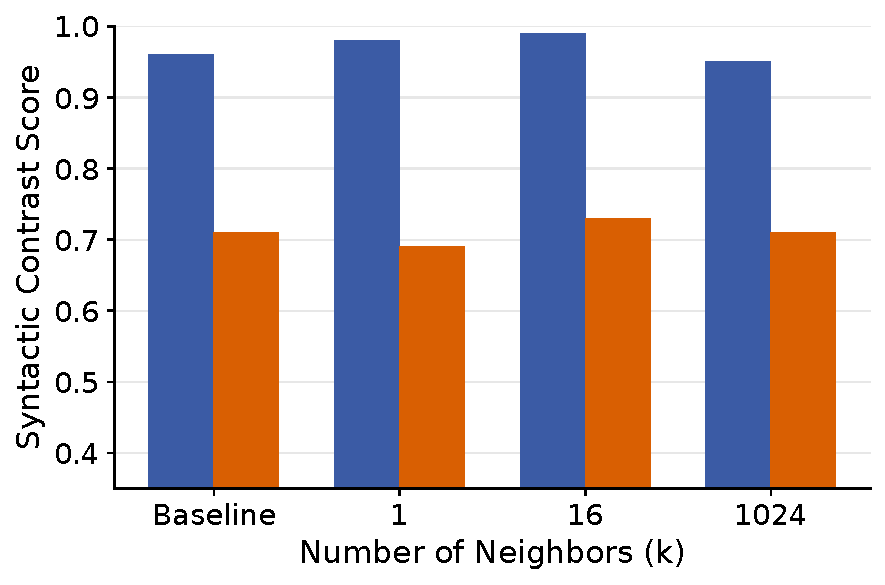
\includegraphics[width=\linewidth]{figs/paper/neighbor/Context10_gpt2-xl_SV_Phrase.pdf}
    (b) SV -- phrase
\end{minipage}\hfill
\begin{minipage}[t]{0.32\textwidth}
    \centering
    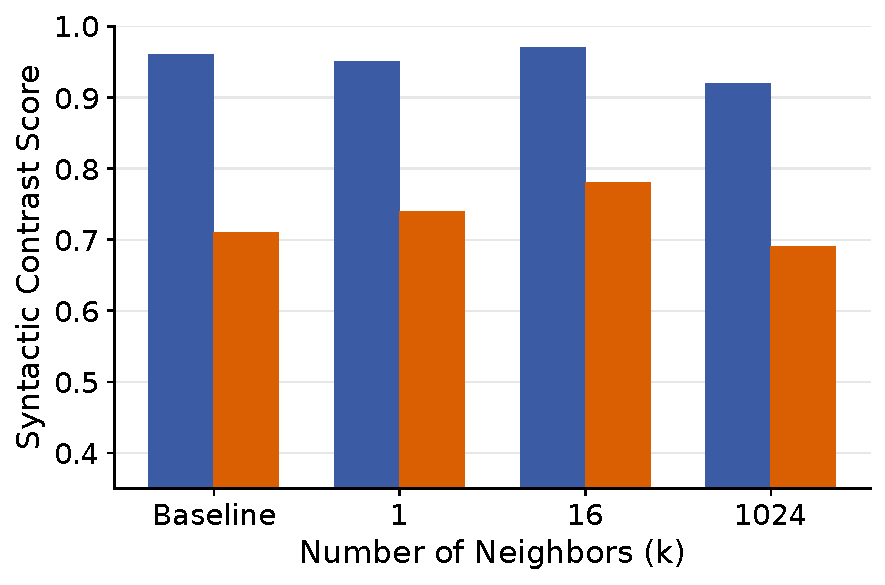
\includegraphics[width=\linewidth]{figs/paper/neighbor/Context10_gpt2-xl_SV_Clause.pdf}
    (c) SV -- sequence
\end{minipage}
\vspace{2mm}
\begin{minipage}[t]{0.32\textwidth}
    \centering
    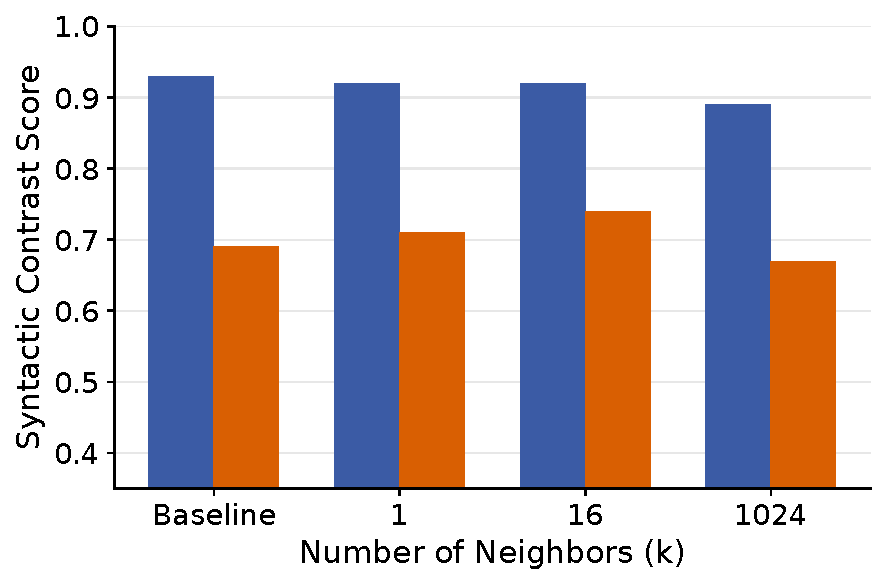
\includegraphics[width=\linewidth]{figs/paper/neighbor/Context10_gpt2-xl_Wh_token.pdf}
    (d) Wh -- token
\end{minipage}\hfill
\begin{minipage}[t]{0.32\textwidth}
    \centering
    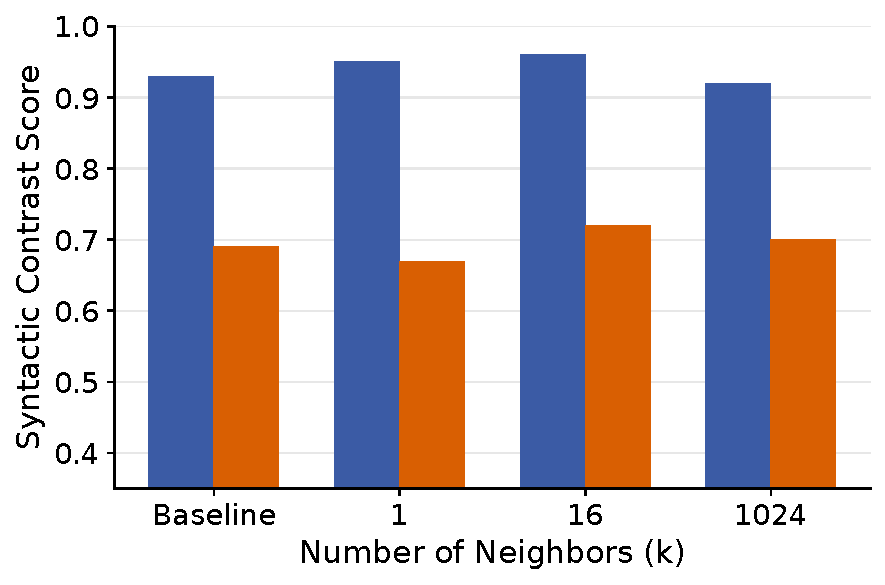
\includegraphics[width=\linewidth]{figs/paper/neighbor/Context10_gpt2-xl_Wh_Phrase.pdf}
    (e) Wh -- phrase
\end{minipage}\hfill
\begin{minipage}[t]{0.32\textwidth}
    \centering
    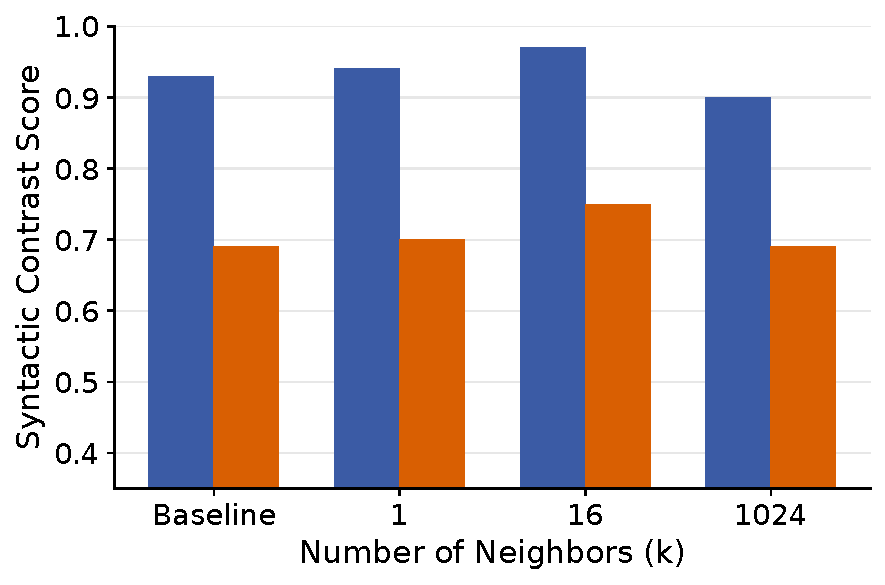
\includegraphics[width=\linewidth]{figs/paper/neighbor/Context10_gpt2-xl_Wh_Clause.pdf}
    (f) Wh -- sequence
\end{minipage}
\vspace{2mm}
\begin{minipage}[t]{0.32\textwidth}
    \centering
    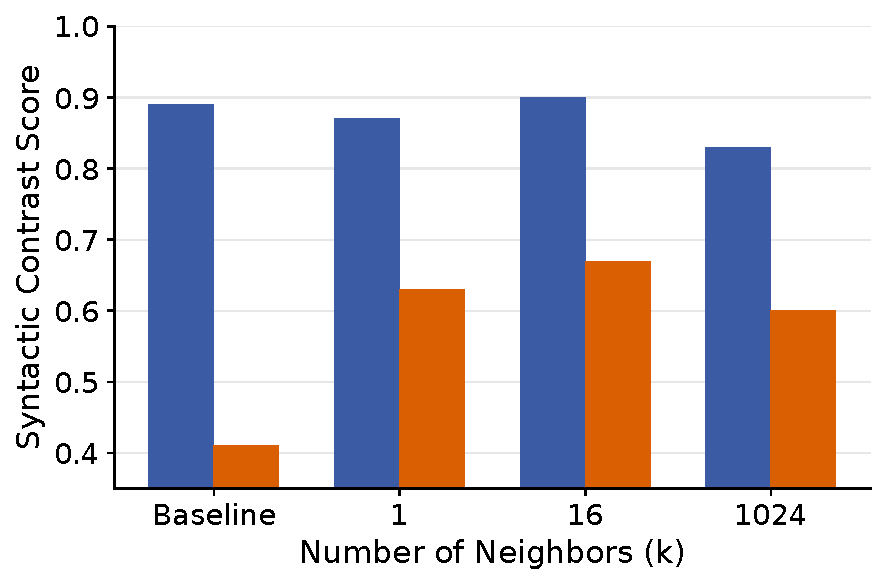
\includegraphics[width=\linewidth]{figs/paper/neighbor/Context10_gpt2-xl_RCs_token.pdf}
    (g) RC -- token
\end{minipage}\hfill
\begin{minipage}[t]{0.32\textwidth}
    \centering
    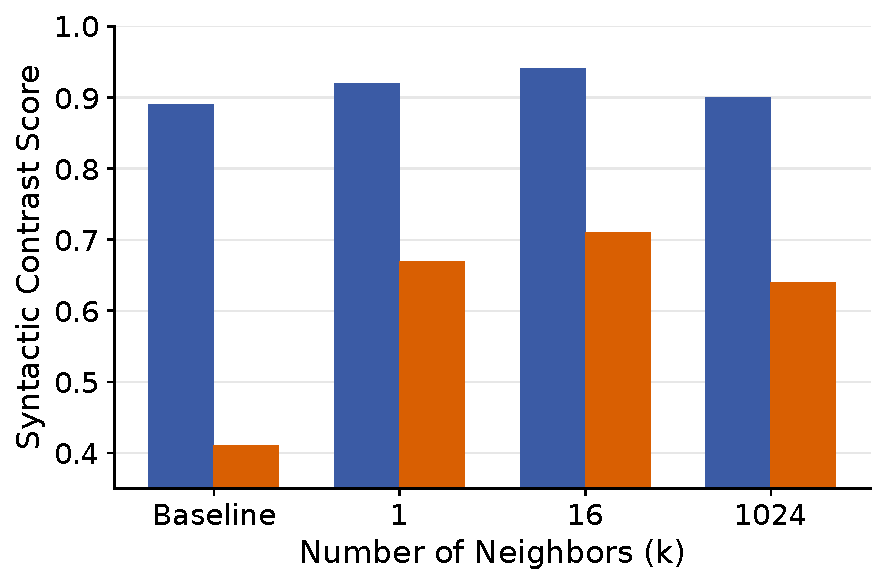
\includegraphics[width=\linewidth]{figs/paper/neighbor/Context10_gpt2-xl_RCs_Phrase.pdf}
    (h) RC -- phrase
\end{minipage}\hfill
\begin{minipage}[t]{0.32\textwidth}
    \centering
    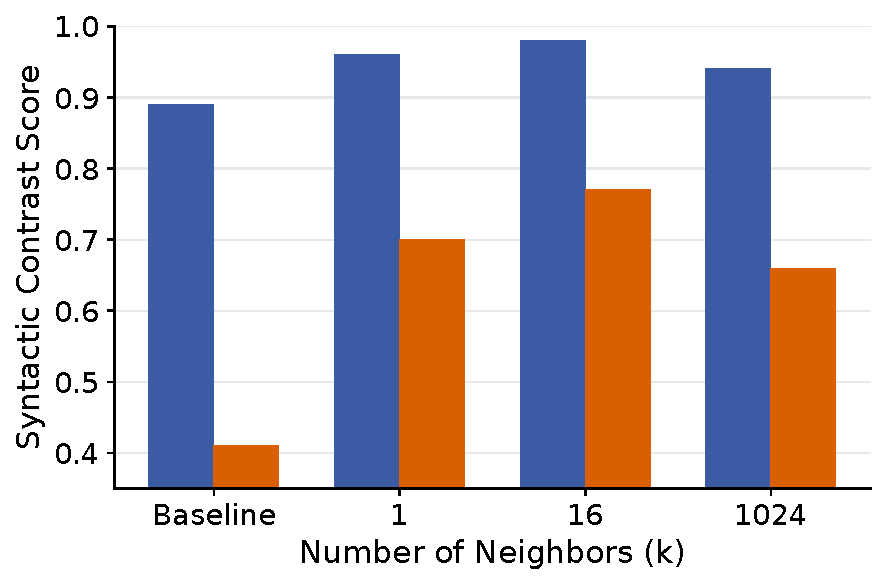
\includegraphics[width=\linewidth]{figs/paper/neighbor/Context10_gpt2-xl_RCs_Clause.pdf}
    (i) RC -- sequence
\end{minipage}
\caption{Effect of number of retrieved neighbors ($k \in \{1,16,1024\}$) for GPT-2 XL at $\tau=10$. Blue bars indicate high-frequency items and orange bars indicate low-frequency items; baseline results are shown for reference.}
\label{fig:app_neighbor_gpt2xl_tau10}
\end{figure*}

% ===== FIGURE: Neighbor count, Bounded-data, tau=1 =====
\begin{figure*}[ht]
\centering
\begin{minipage}[t]{0.32\textwidth}
    \centering
    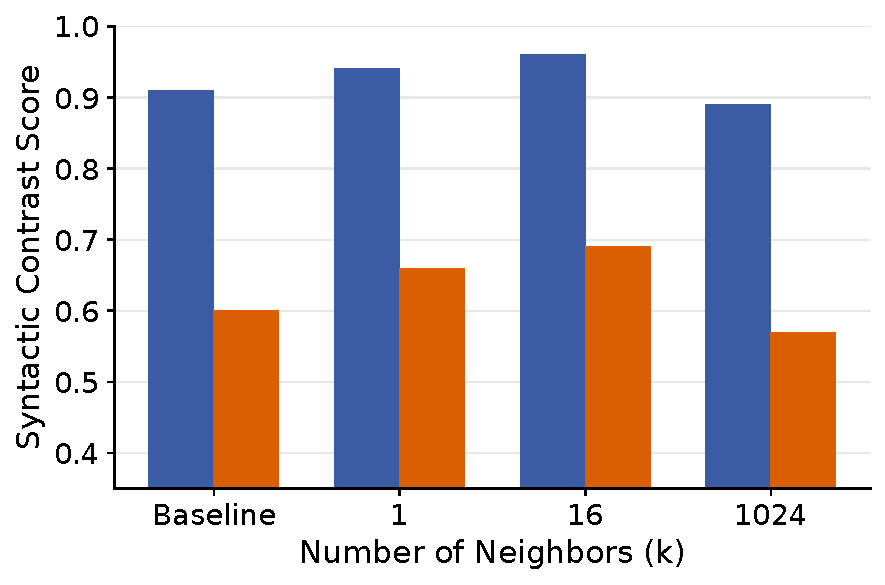
\includegraphics[width=\linewidth]{figs/paper/neighbor/Context1_child-realistic_SV_token.pdf}
    (a) SV -- token
\end{minipage}\hfill
\begin{minipage}[t]{0.32\textwidth}
    \centering
    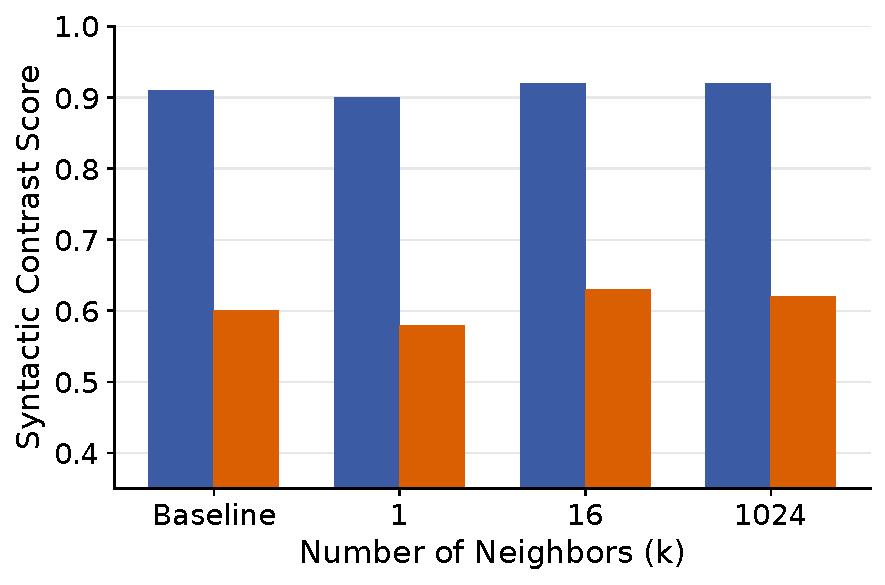
\includegraphics[width=\linewidth]{figs/paper/neighbor/Context1_child-realistic_SV_Phrase.pdf}
    (b) SV -- phrase
\end{minipage}\hfill
\begin{minipage}[t]{0.32\textwidth}
    \centering
    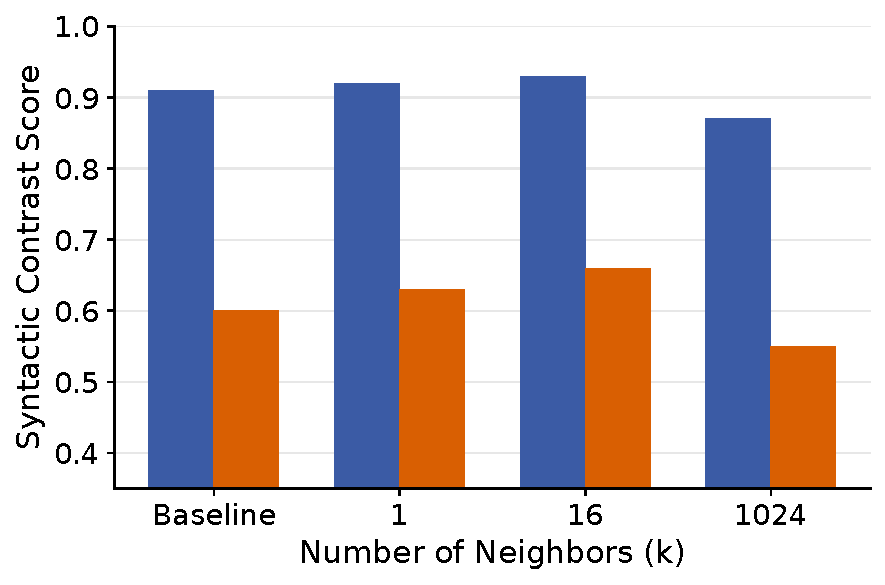
\includegraphics[width=\linewidth]{figs/paper/neighbor/Context1_child-realistic_SV_Clause.pdf}
    (c) SV -- sequence
\end{minipage}
\vspace{2mm}
\begin{minipage}[t]{0.32\textwidth}
    \centering
    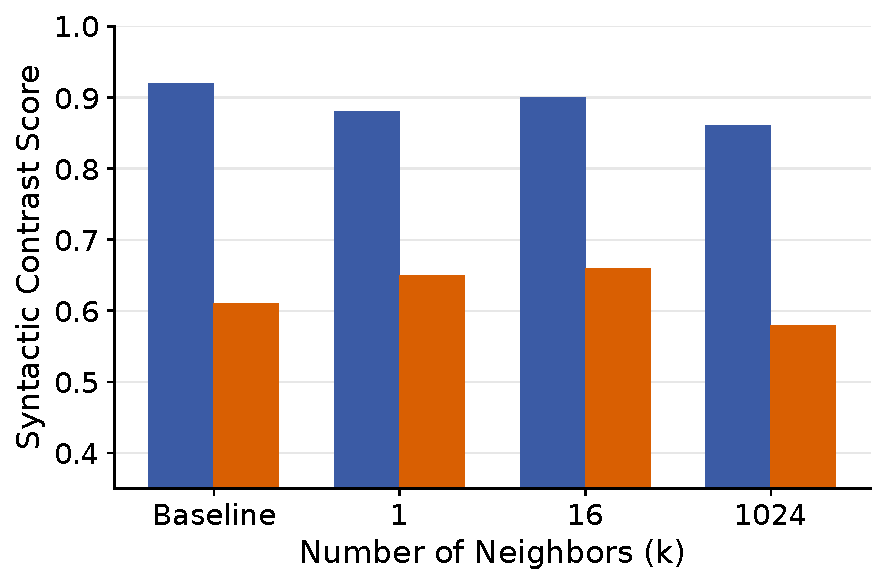
\includegraphics[width=\linewidth]{figs/paper/neighbor/Context1_child-realistic_Wh_token.pdf}
    (d) Wh -- token
\end{minipage}\hfill
\begin{minipage}[t]{0.32\textwidth}
    \centering
    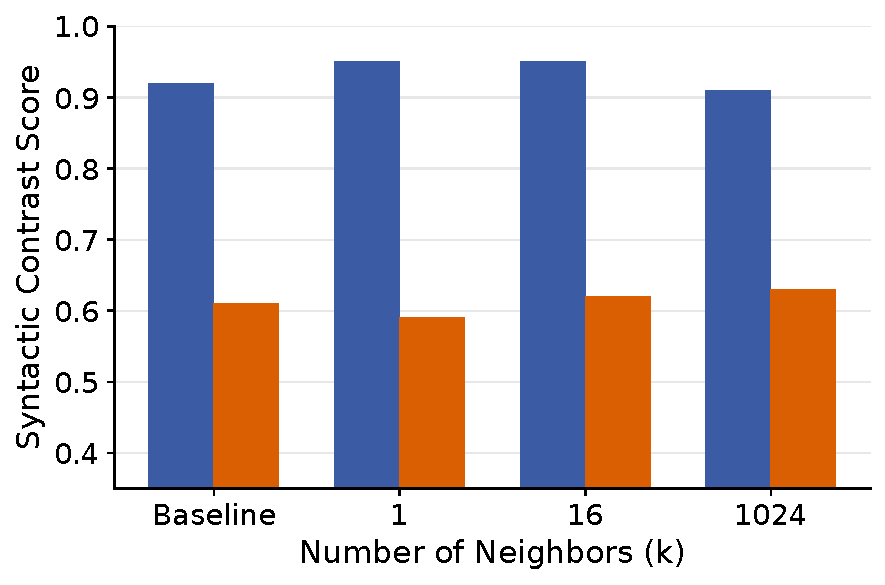
\includegraphics[width=\linewidth]{figs/paper/neighbor/Context1_child-realistic_Wh_Phrase.pdf}
    (e) Wh -- phrase
\end{minipage}\hfill
\begin{minipage}[t]{0.32\textwidth}
    \centering
    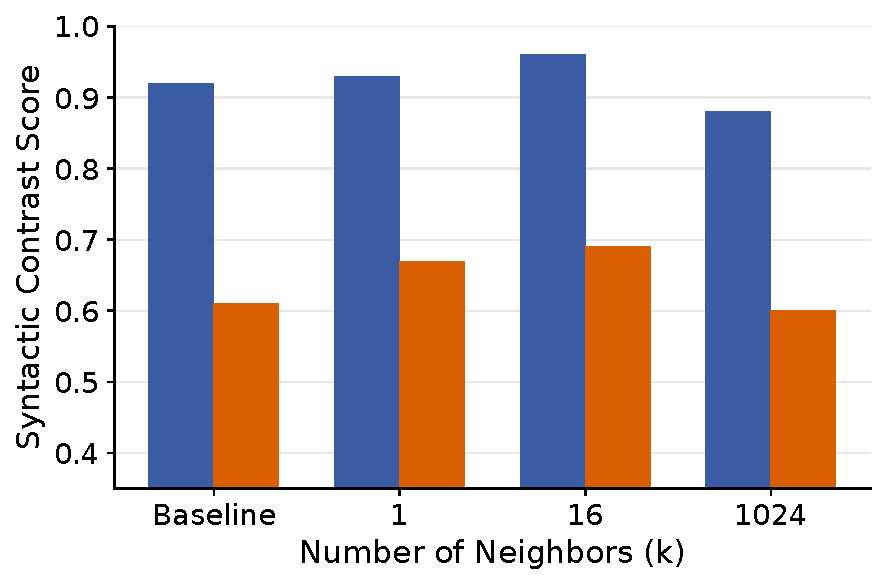
\includegraphics[width=\linewidth]{figs/paper/neighbor/Context1_child-realistic_Wh_Clause.pdf}
    (f) Wh -- sequence
\end{minipage}
\vspace{2mm}
\begin{minipage}[t]{0.32\textwidth}
    \centering
    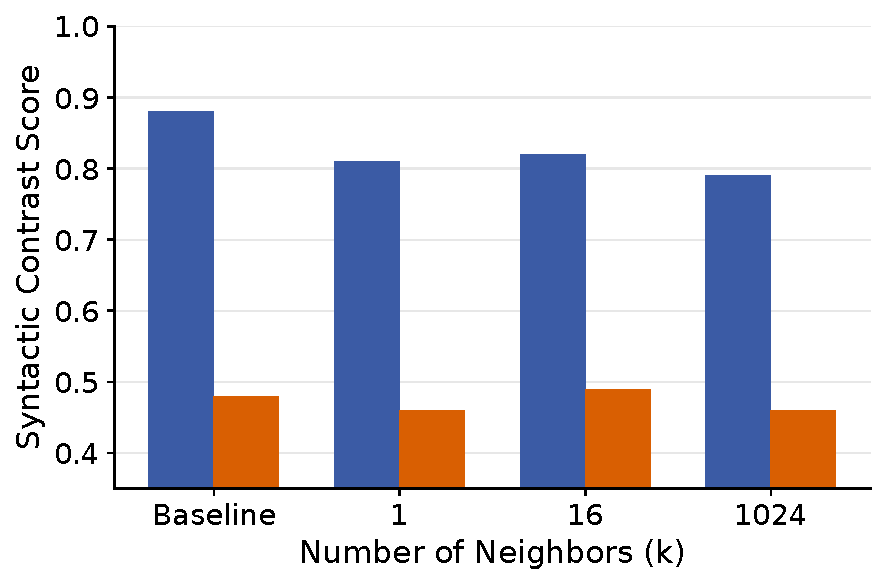
\includegraphics[width=\linewidth]{figs/paper/neighbor/Context1_child-realistic_RCs_token.pdf}
    (g) RC -- token
\end{minipage}\hfill
\begin{minipage}[t]{0.32\textwidth}
    \centering
    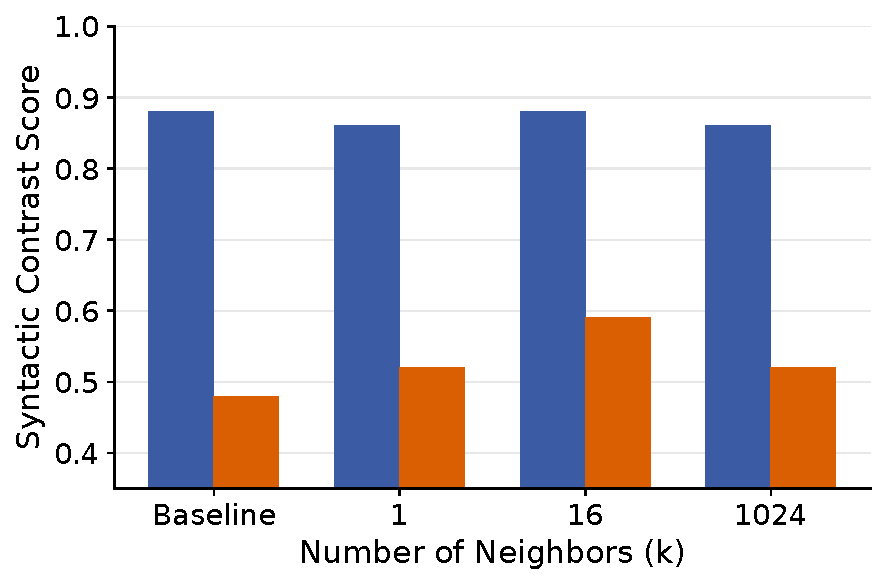
\includegraphics[width=\linewidth]{figs/paper/neighbor/Context1_child-realistic_RCs_Phrase.pdf}
    (h) RC -- phrase
\end{minipage}\hfill
\begin{minipage}[t]{0.32\textwidth}
    \centering
    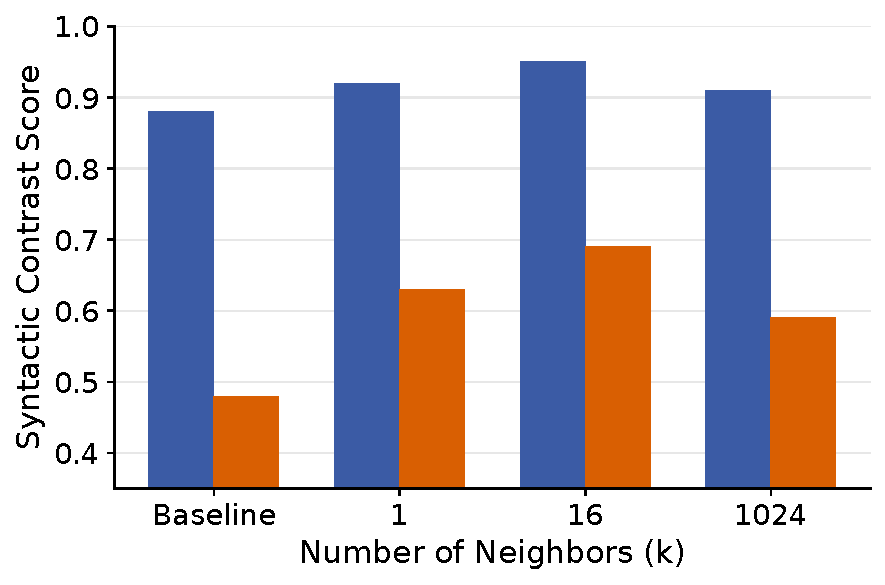
\includegraphics[width=\linewidth]{figs/paper/neighbor/Context1_child-realistic_RCs_Clause.pdf}
    (i) RC -- sequence
\end{minipage}
\caption{Effect of number of retrieved neighbors ($k \in \{1,16,1024\}$) for the bounded-data model at $\tau=1$. Blue bars indicate high-frequency items and orange bars indicate low-frequency items; baseline results are shown for reference.}
\label{fig:app_neighbor_child_tau1}
\end{figure*}

% ===== FIGURE: Neighbor count, Bounded-data, tau=10 =====
\begin{figure*}[ht]
\centering
\begin{minipage}[t]{0.32\textwidth}
    \centering
    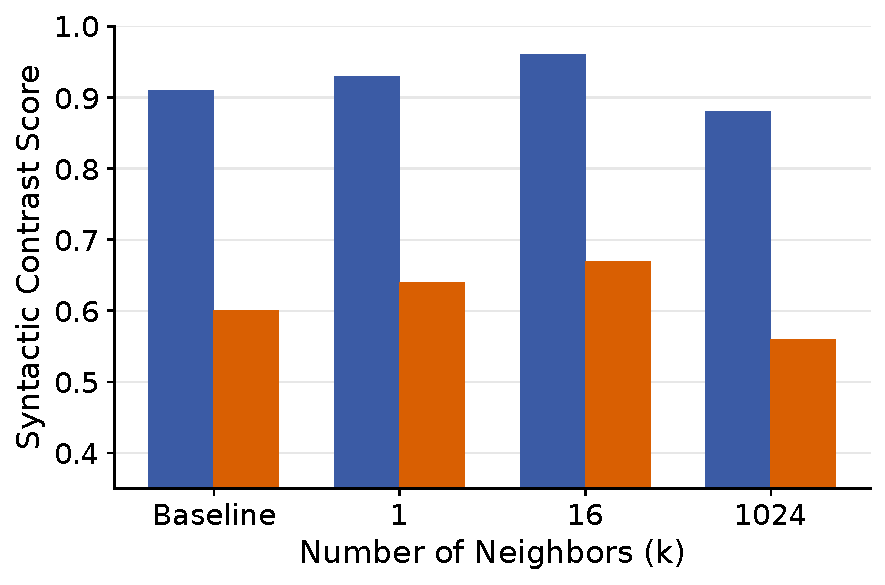
\includegraphics[width=\linewidth]{figs/paper/neighbor/Context10_child-realistic_SV_token.pdf}
    (a) SV -- token
\end{minipage}\hfill
\begin{minipage}[t]{0.32\textwidth}
    \centering
    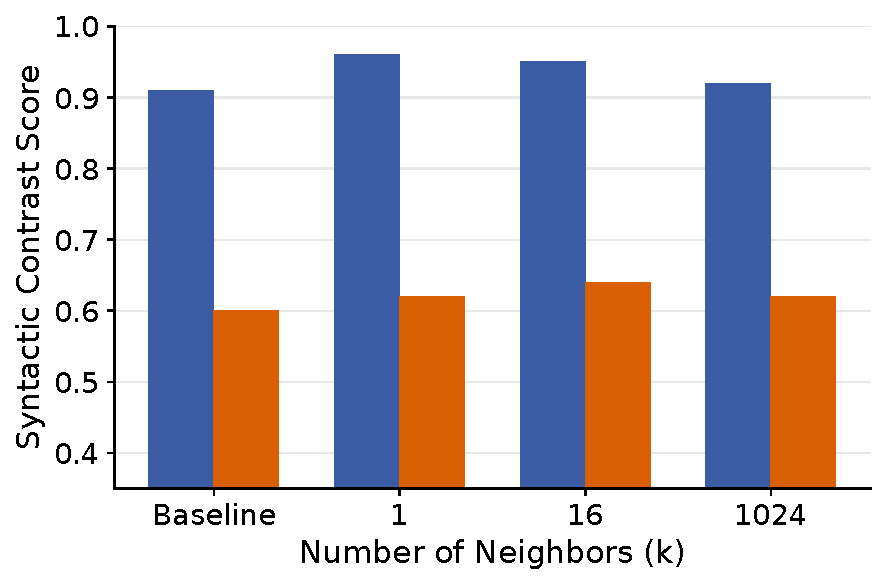
\includegraphics[width=\linewidth]{figs/paper/neighbor/Context10_child-realistic_SV_Phrase.pdf}
    (b) SV -- phrase
\end{minipage}\hfill
\begin{minipage}[t]{0.32\textwidth}
    \centering
    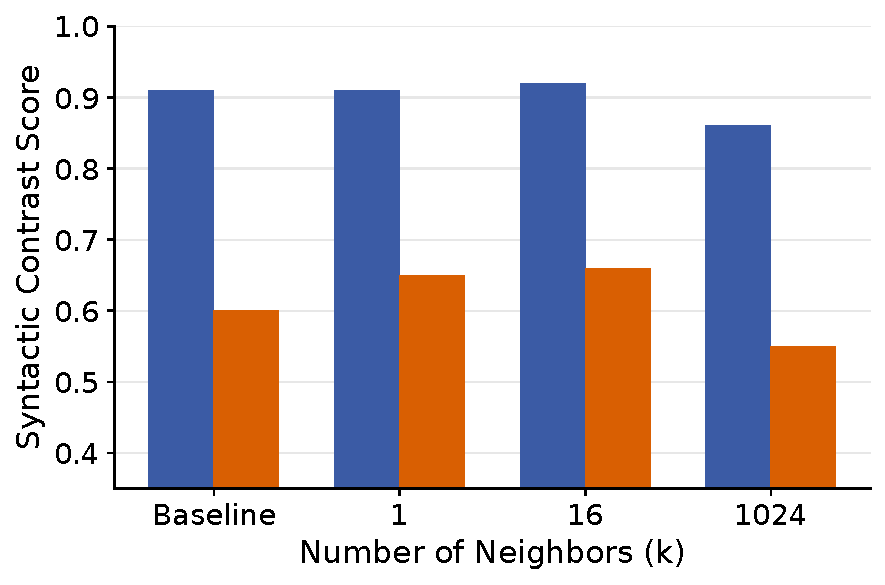
\includegraphics[width=\linewidth]{figs/paper/neighbor/Context10_child-realistic_SV_Clause.pdf}
    (c) SV -- sequence
\end{minipage}
\vspace{2mm}
\begin{minipage}[t]{0.32\textwidth}
    \centering
    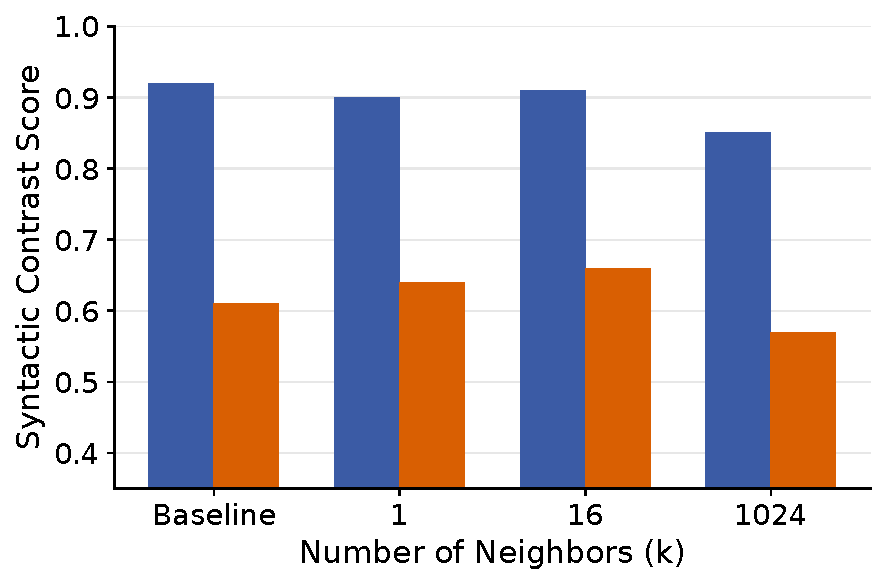
\includegraphics[width=\linewidth]{figs/paper/neighbor/Context10_child-realistic_Wh_token.pdf}
    (d) Wh -- token
\end{minipage}\hfill
\begin{minipage}[t]{0.32\textwidth}
    \centering
    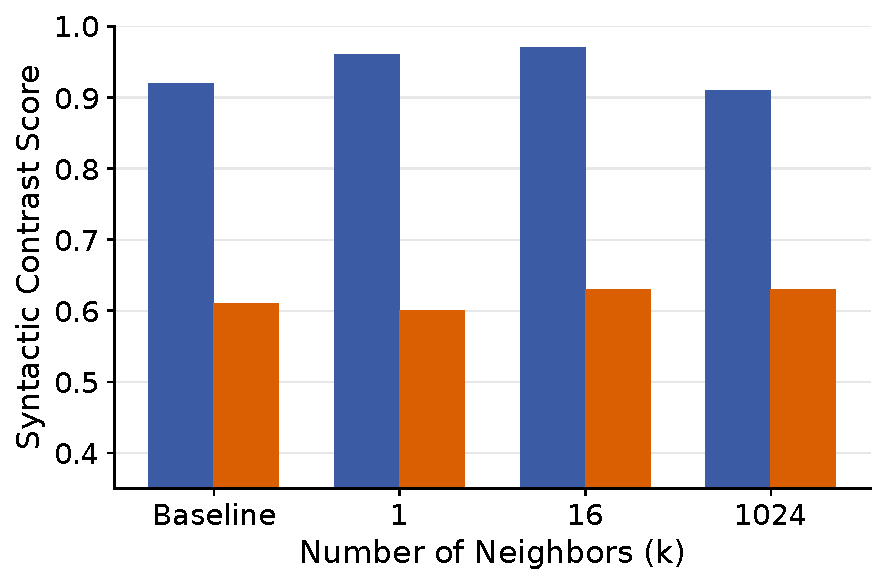
\includegraphics[width=\linewidth]{figs/paper/neighbor/Context10_child-realistic_Wh_Phrase.pdf}
    (e) Wh -- phrase
\end{minipage}\hfill
\begin{minipage}[t]{0.32\textwidth}
    \centering
    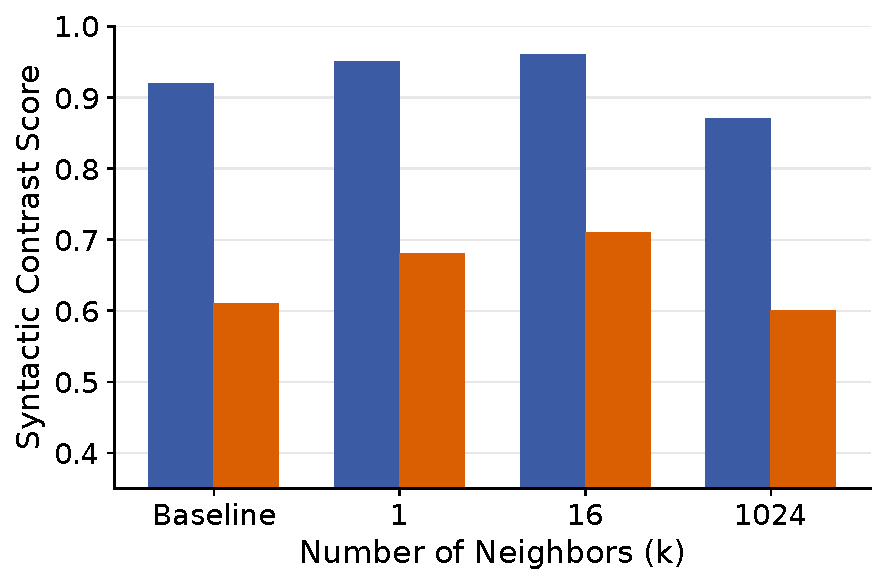
\includegraphics[width=\linewidth]{figs/paper/neighbor/Context10_child-realistic_Wh_Clause.pdf}
    (f) Wh -- sequence
\end{minipage}
\vspace{2mm}
\begin{minipage}[t]{0.32\textwidth}
    \centering
    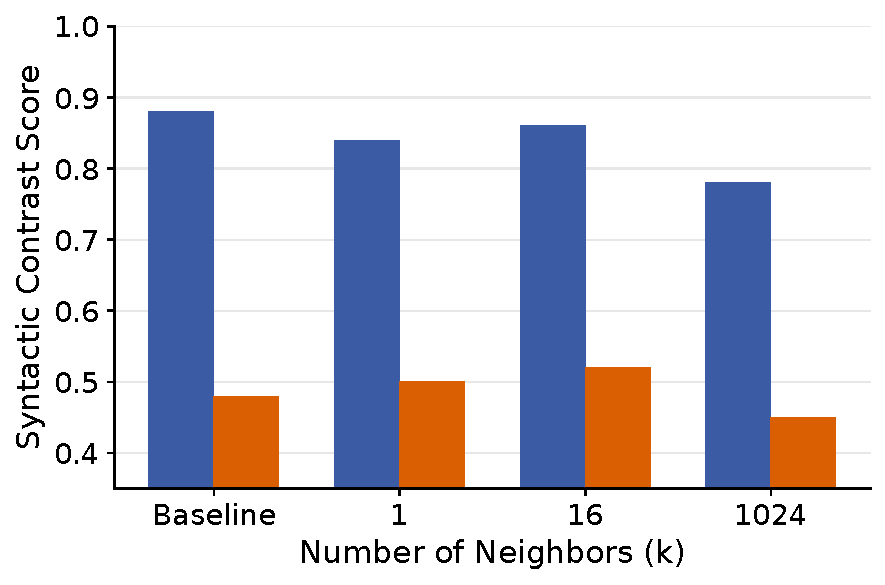
\includegraphics[width=\linewidth]{figs/paper/neighbor/Context10_child-realistic_RCs_token.pdf}
    (g) RC -- token
\end{minipage}\hfill
\begin{minipage}[t]{0.32\textwidth}
    \centering
    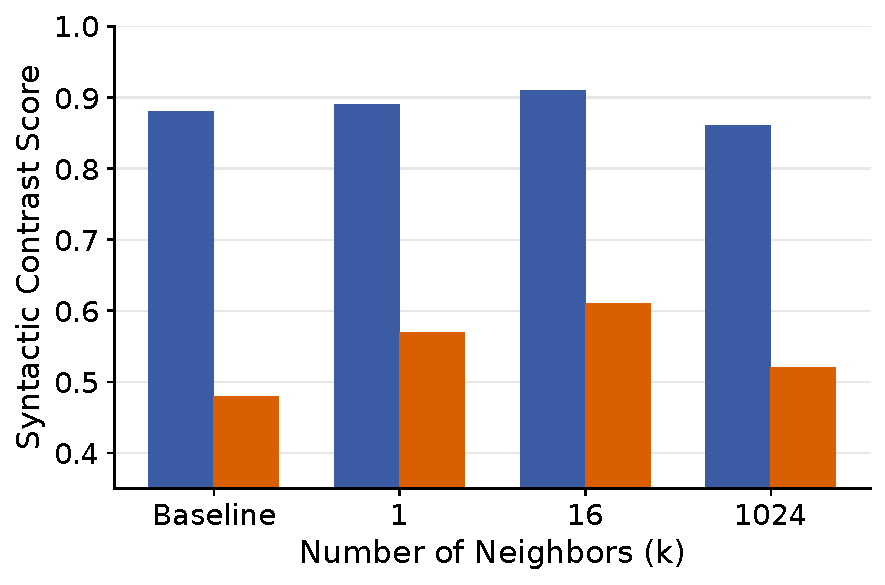
\includegraphics[width=\linewidth]{figs/paper/neighbor/Context10_child-realistic_RCs_Phrase.pdf}
    (h) RC -- phrase
\end{minipage}\hfill
\begin{minipage}[t]{0.32\textwidth}
    \centering
    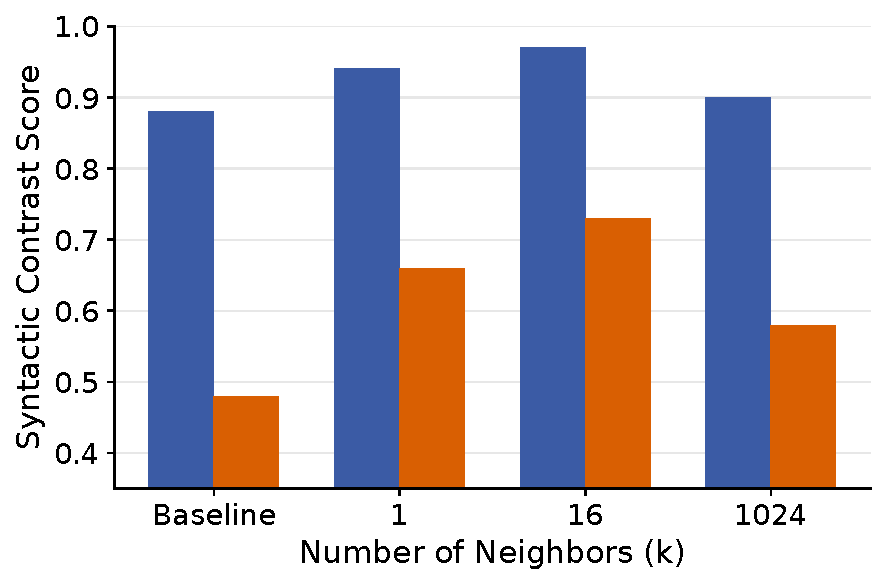
\includegraphics[width=\linewidth]{figs/paper/neighbor/Context10_child-realistic_RCs_Clause.pdf}
    (i) RC -- sequence
\end{minipage}
\caption{Effect of number of retrieved neighbors ($k \in \{1,16,1024\}$) for the bounded-data model at $\tau=10$. Blue bars indicate high-frequency items and orange bars indicate low-frequency items; baseline results are shown for reference.}
\label{fig:app_neighbor_child_tau10}
\end{figure*}






\clearpage
\endgroup
